\chapter{Methods}
\label{chapter2}
\justifying
% Have a section for each paper
% Have lot's of graphs and images

% short summary of your method, 1 to 2 paragraphs
% the three sections on the three papers
% implementation details, for example, you can break it down into steps like how you did on reddit
% ps: use as many figure to show your work as possible
% figures include: at least one illustration on how your method work and as many figures on the ocean as possible

\section{Algorithm Overview}

\begin{minipage}{1\textwidth}
    \centering
    \includegraphics[width=0.8\textwidth]{"images/ocean_algorithm.png"}
    \captionof{figure}{Ocean Generation Algorithm Stages: (1) Gaussian Noise Generation, (2) Initial Spectrum Creation, (3) Frequency Map Production, and (4) Conversion to Time Domain via IFFT.}
    \label{fig:ocean_algorithm}
\end{minipage}
\vspace{0.0cm}

The ocean generation algorithm utilizes the Fast Fourier Transform (FFT) and is designed for the Unity engine. It uses the High-Level Shader Language (HLSL) for GPU computations. The algorithm processes textures of size $N$x$N$, with N being a power of 2, to satisfy the Inverse Fast Fourier Transform (IFFT) data sample requirement. For this project, we use a texture size of 512x512, balancing computational performance and visual realism. The algorithm comprises four main stages, as shown in Figure \ref{fig:ocean_algorithm}.

\begin{enumerate}
    \item \textbf{Gaussian Noise Generation:} The first stage involves the generation of Gaussian noise with a mean of 0 and a standard deviation of 1. Two values are generated, one for the real part and the other for the complex part, as shown in Equation \ref{eq:fouier_amplitudes}.
    \item \textbf{Spectrum Generation:} The second stage involves the generation of the initial spectrum, $\tilde{h}_0(\mathbf{k})$, which is used to generate all subsequent results. The real and imaginary parts of the spectrum are stored as the red and green channels of a texture, respectively. Additionally, a separate texture is used to store the wave vector, $\mathbf{k}$, and the dispersion relation, $\omega$.
    \item \textbf{Frequency Generation:} In the third stage, the initial spectrum is used to generate a frequency height map for vertical vertex displacement, a frequency normal map for shading, and a frequency horizontal displacement map for horizontal vertex displacement. Furthermore, six values are calculated for the Jacobian, which is used to generate foam. Due to the limitation of a maximum of four values per texture, two textures are used to store the Jacobian values.
    \item \textbf{Inverse FFT (IFFT) Conversion:} The final stage involves the use of the Inverse Fast Fourier Transform (IFFT) algorithm to convert the maps from the frequency domain to the time domain.
\end{enumerate}

\section{IFFT}

\begin{minipage}{1\textwidth}
    \centering
    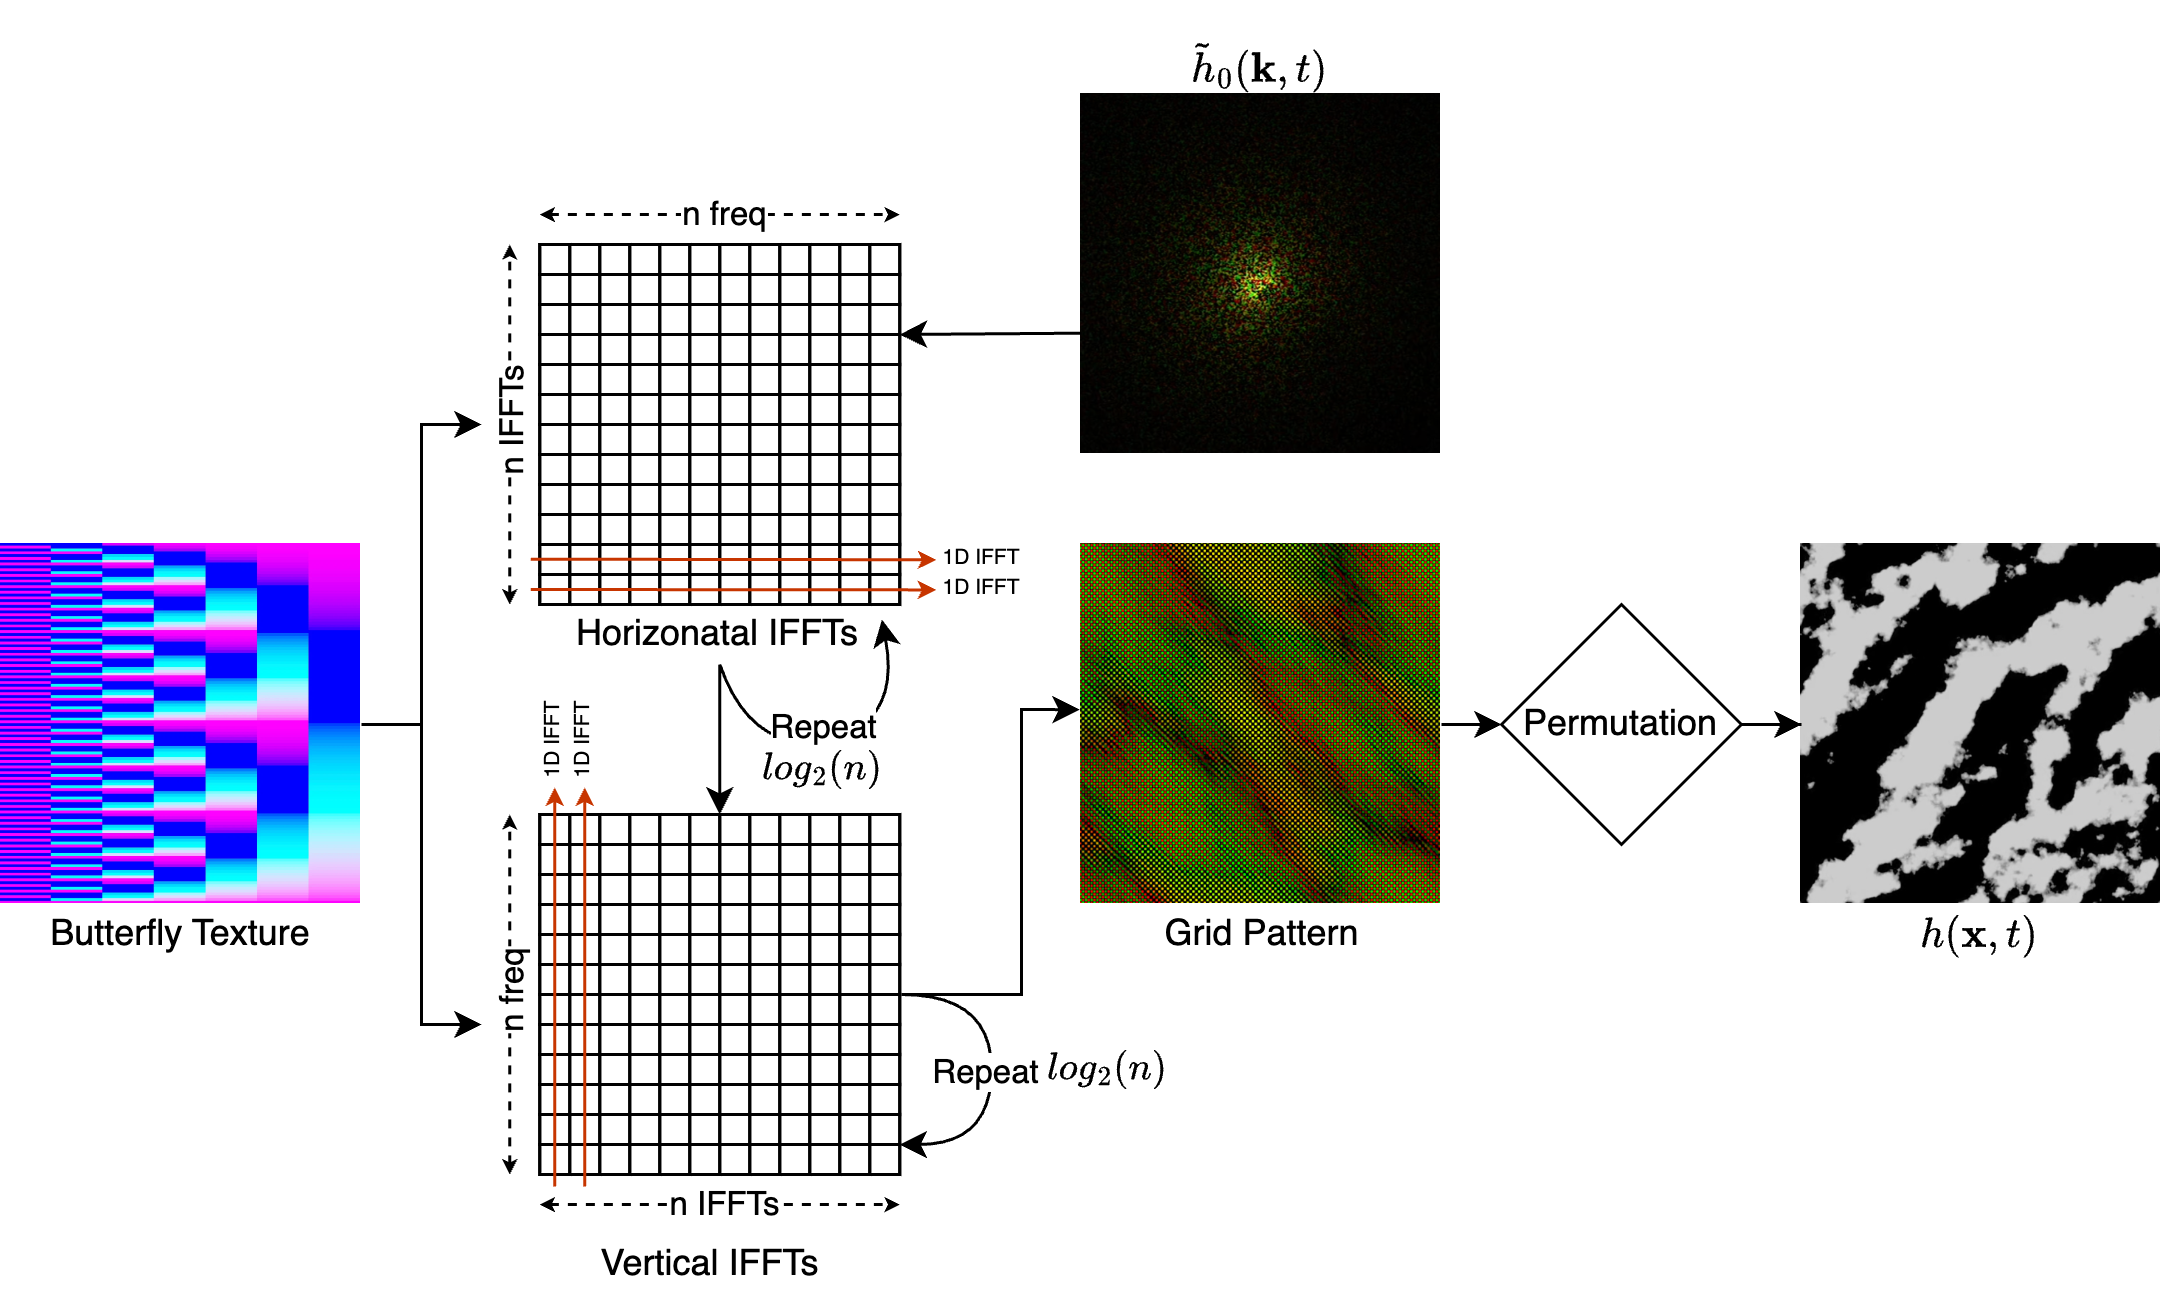
\includegraphics[width=1\textwidth]{"images/ifft_algorithm.png"}
    \captionof{figure}{During the initialization phase, we generate a butterfly texture that stores the twiddle factors and indices. Subsequently, we apply a horizontal IFFT to the signal of size $n_2$, repeating this process $\log_2(n)$ times. The same procedure is then applied to vertical IFFT. Finally, we permute the data to transition from the frequency domain to the time domain.}
    \label{fig:ifft_algorithm}
\end{minipage}

\subsection{Butterfly Texture}

Our focus is primarily on the Inverse Fast Fourier Transform (IFFT) algorithm, and we will not be utilizing the FFT. To execute the IFFT, we generate a butterfly texture, as proposed by Fl{\"u}gge Fynn-Jorin (2017) \cite{flugge2017}. This texture, which is precomputed and stored in the GPU memory, has a width of $\log_2(n)$ and a height of n. It is a four-channel texture $(W_r,W_i,y_t,y_b)$, where $W_r$ and $W_i$ are the real and imaginary parts of the twiddle factor, and $y_t$ and $y_b$ are the top and bottom butterfly indices, respectively (as shown in Figure \ref{fig:butterfly_diagram}).

In butterfly texture coordinate x represents a stage \ref{fig:8_butterfly_diagram}, while each y represents a butterfly operation between two data points $y_t$ and $y_b$.

In the first stage we sort our data in bit reversed order, In the subsequent stages, we perform the following operations:
\begin{itemize}
    \item If the butterfly wing is top half as shown in \ref{fig:8_butterfly_diagram}
    \begin{equation}
        \begin{split}
            y_t &= y_{\text{current}} \\
            y_b &= y_{\text{current}} + 2^{\text{stage}}
        \end{split}
    \end{equation}
    \item If the butterfly wing is bottom half
    \begin{equation}
        \begin{split}
            y_t &= y_{\text{current}} - 2^{\text{stage}} \\
            y_b &= y_{\text{current}}
        \end{split}
    \end{equation}
\end{itemize}
We can determine whether the wing is in the upper or lower half using the following equation:
\begin{equation}
    \text{wing} = y_{\text{current}} \bmod 2^{(\text{stage} + 1)}
\end{equation}
Finally, we calculate the twiddle factors as follows:
\begin{equation}
    \begin{split}
        k &= (y_{\text{current}} \cdot n / 2^{\text{stage} + 1}) \bmod n \\
        W &= \exp(-2\pi i k / n)
    \end{split}
\end{equation}

\subsection{Performing IFFT}
Our data is currently stored in a 2D texture. However, the IFFT algorithm is designed for 1D data. As a result, we need to perform a 1D IFFT on each row (horizontally) and then on each column (vertically), as shown in Figure \ref{fig:ifft_algorithm}.
By following pseudocode proposed by Fl{\"u}gge Fynn-Jorin (2017) \cite{flugge2017} we can perform IFFT in 2D:

\begin{lstlisting}[caption={Horizontal Butterfly Operation}, frame=single, numberstyle=\small\color{gray}, captionpos=b]
    butterflyData = ButterflyTexture[Stage, id.x];
    twiddle = butterflyData.xy;
    // fetch top butterfly input sample
    topSignal = PingPong0[butterflyData.z, id.y].xy;
    // fetch bottom butterfly input sample
    bottomSignal = PingPong0[butterflyData.w, id.y].xy;
    // perform butterfly operation
    h = topSignal + ComplexMult(twiddle, bottomSignal);
\end{lstlisting}

Notice that we are using ping-pong buffers to store intermediate results, as we need to perform multiple IFFT passes, in total $log_2(n)$ passes.
After we perform IFFT on each row, we need to perform for each column:
\begin{lstlisting}[caption={Vertical Butterfly Operation}, frame=single, numberstyle=\small\color{gray}, captionpos=b]
    butterflyData = ButterflyTexture[Stage, id.y];
    twiddle = butterflyData.xy;
    // fetch top butterfly input sample
    topSignal = PingPong0[id.x, butterflyData.z].xy;
    // fetch bottom butterfly input sample
    bottomSignal = PingPong0[id.x, butterflyData.w].xy;
    // perform butterfly operation
    h = topSignal + ComplexMult(twiddle, bottomSignal);
\end{lstlisting}

\subsection*{Permutation}
Lastlly, our data needs to be permuted as you will see later our data is offseted:
\begin{equation}
    [\text{freq} (-N / 2), \text{ ...}, \text{ freq} (-1), \text{ freq} (0), \text{ freq} (1), \text{ ...}, \text{ freq} (N / 2 - 1)]
\end{equation}
While, our IFFT algorithm expected data to be in the following order:
\begin{equation}
    [\text{freq} (0), \text{ freq} (1), \text{ ...}, \text{ freq}(N - 1)]
\end{equation}
This causes our data to flip sign in grid like pattern therefore we need to permute our data:
\begin{lstlisting}[caption={Data Permutation \cite{flugge2017} }, frame=single, numberstyle=\small\color{gray}, captionpos=b]
    signs = {-1, 1};
    index = (id.x + id.y) % 2;
    sign = signs[index];
    h = sign * PingPong1[id.xy].x;
    
    PingPong0[id.xy] = h
\end{lstlisting}

\section{Ocean Geometry}
% Table
\begin{table}[H]
    \centering
    \begin{tabular}{cl}
        \toprule
        \textbf{Symbol} & \textbf{Meaning} \\
        \midrule
        $S(\omega)$ & Non directional wave spectrum \\
        $S(\omega, \theta)$ & Directional wave spectrum\\
        $S(\mathbf{k})$ & Directional wave spectrum\\
        $\mathbf{k}$ & wave vector \\
        $k$ & Magnetude of wave vector\\
        $l$ & Length scale of the ocean\\
        $\omega$ & dispertion relationship (angular frequency)\\
        $U_{10}$ & Wind speed at 10m above the sea level\\
        $F$ & Fetch (Disntance from lee shore)\\
        $\theta_{\text{wind}}$ & Wind angle\\
        $\lambda$ & Wave Choppy factor\\
        \bottomrule
    \end{tabular}
    \caption{Deffinition Table}
    \label{table:deffinition_table}
\end{table}

\subsection{Spectrum Generation}

\begin{minipage}{1\textwidth}
    \centering
    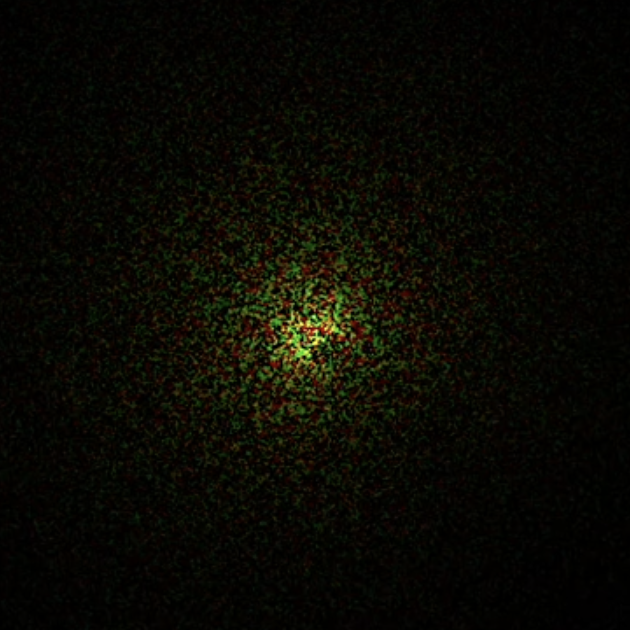
\includegraphics[width=0.40\textwidth]{"images/tma_spectrum.png"}
    \captionof{figure}{TMA spectrum, Frequency Domain}
    \label{fig:tma_spectrum}
\end{minipage}
\vspace{0cm}

The choice of spectrum is pivotal to the visual fidelity of an ocean simulation. The Tessendorf's spectrum, initially implemented due to its straightforward application, did not yield satisfactory results. The wave energy transfer was unconvincing, the waves did not appear to adhere to the wave direction, and artistic control over the ocean's appearance was challenging. To ensure the realism of the simulated ocean, the TMA spectrum \ref{eq:tma_spectrum_k}, grounded in empirical data, was subsequently implemented:
$$
    S_{\text{TMA}}(\mathbf{k}) = 2S_{\text{TMA}}(\omega, h) \cdot \frac{d\omega}{dk} / k \cdot \Delta k_x \cdot \Delta k_y
$$
where $\mathbf{k} = (k_x, k_y)$, $k_x = 2 * \pi (x_x - n/2)/ l$, $k_y = 2 * \pi (x_y - n/2)/ l$, $l$ is the the length scale of the ocean, 
and $\mathbf{x} = (x_x, x_y)$ is current position in the texture. 

The TMA spectrum \ref{fig:tma_spectrum} resulted in a more realistic ocean simulation, offering intuitive controls over fetch, wind speed, wind angle, and depth. It required minimal effort to achieve a realistic appearance and provided satisfactory results out of the box.

\subsection{Height Map Generation}

\begin{minipage}{1\textwidth}
    \centering
    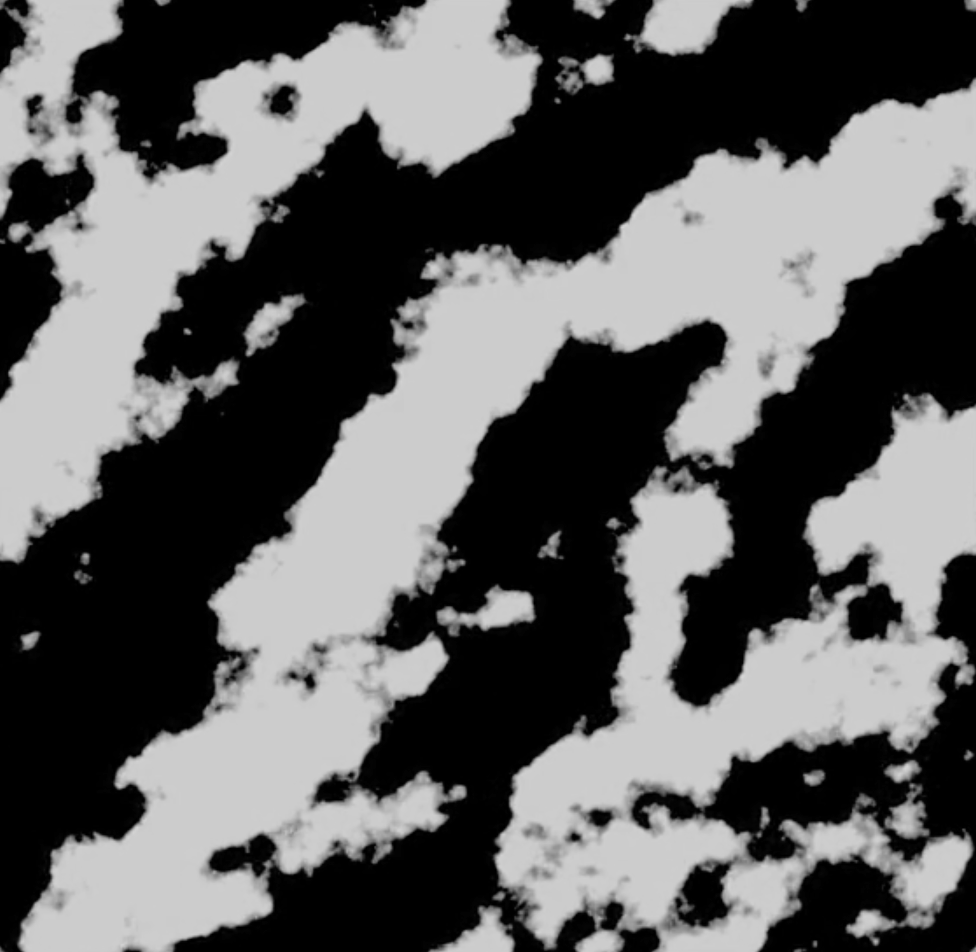
\includegraphics[width=0.40\textwidth]{"images/tma_height.png"}
    \captionof{figure}{Height Map using $S_{\text{TMA}}$}
    \label{fig:tma_height_map}
\end{minipage}

The generation of a height map begins with the computation of Fourier amplitudes, as shown in Equation \ref{eq:fouier_amplitudes}. Here, $P_h$ represents the TMA Spectrum $S_{TMA}(\mathbf{k})$.
The symmetry of the Fourier series allows us to mirror the amplitudes, eliminating the need for complex conjugate recalculation. This is represented as:
\begin{equation}
    \tilde{h}^{*}_0 = T_{h_0}(x^{*}, y^{*})
\end{equation}
where $T_{h_0}(x, y)$ is fourier amplitude in precomputed texture at $x^{*} = (n - x) \text{ mod } n$, $y^{*} = (n - y) \text{ mod } n$, $(x, y)$ is current position in the texture.

By having combined amplitudes \ref{eq:combined_amplitudes} we can perform IFFT as shown in \ref{fig:ifft_algorithm} to produce height map as shown in figure \ref{fig:tma_height_map}.

\subsection{Normal Map Generation}
\begin{minipage}{1\textwidth}
    \centering
    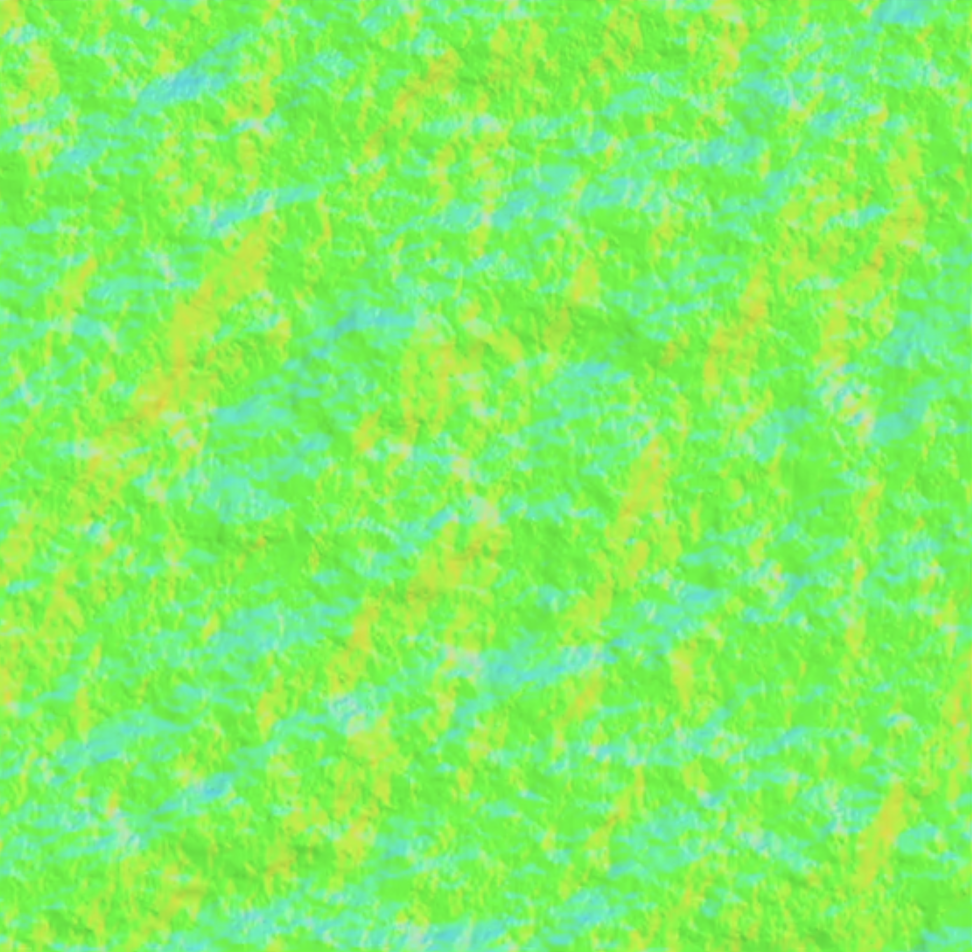
\includegraphics[width=0.40\textwidth]{"images/tma_normal.png"}
    \captionof{figure}{Normal Map using $S_{\text{TMA}}$}
    \label{fig:tma_normal_map}
\end{minipage}

The generation of a normal map is an essential step in ocean simulation as it provides critical information for calculating ocean shading. A normal map represents the perpendicular direction to the ocean surface at each point.
The computation of a normal map necessitates the calculation of the gradient, which is the derivative of the height map. As per Tessendorf (2001) \cite{tessendorf2001}, the derivative is given by:
\begin{equation}
    \epsilon(\textbf{x}, t) = i\textbf{k} \tilde{h}(\textbf{k}, t)
\end{equation}
Then we need to perform IFFT \ref{fig:ifft_algorithm} to get normal map \ref{fig:tma_normal_map} in the time domain.

\subsection{Choppy Waves}
\begin{minipage}{0.49\textwidth}
    \centering
    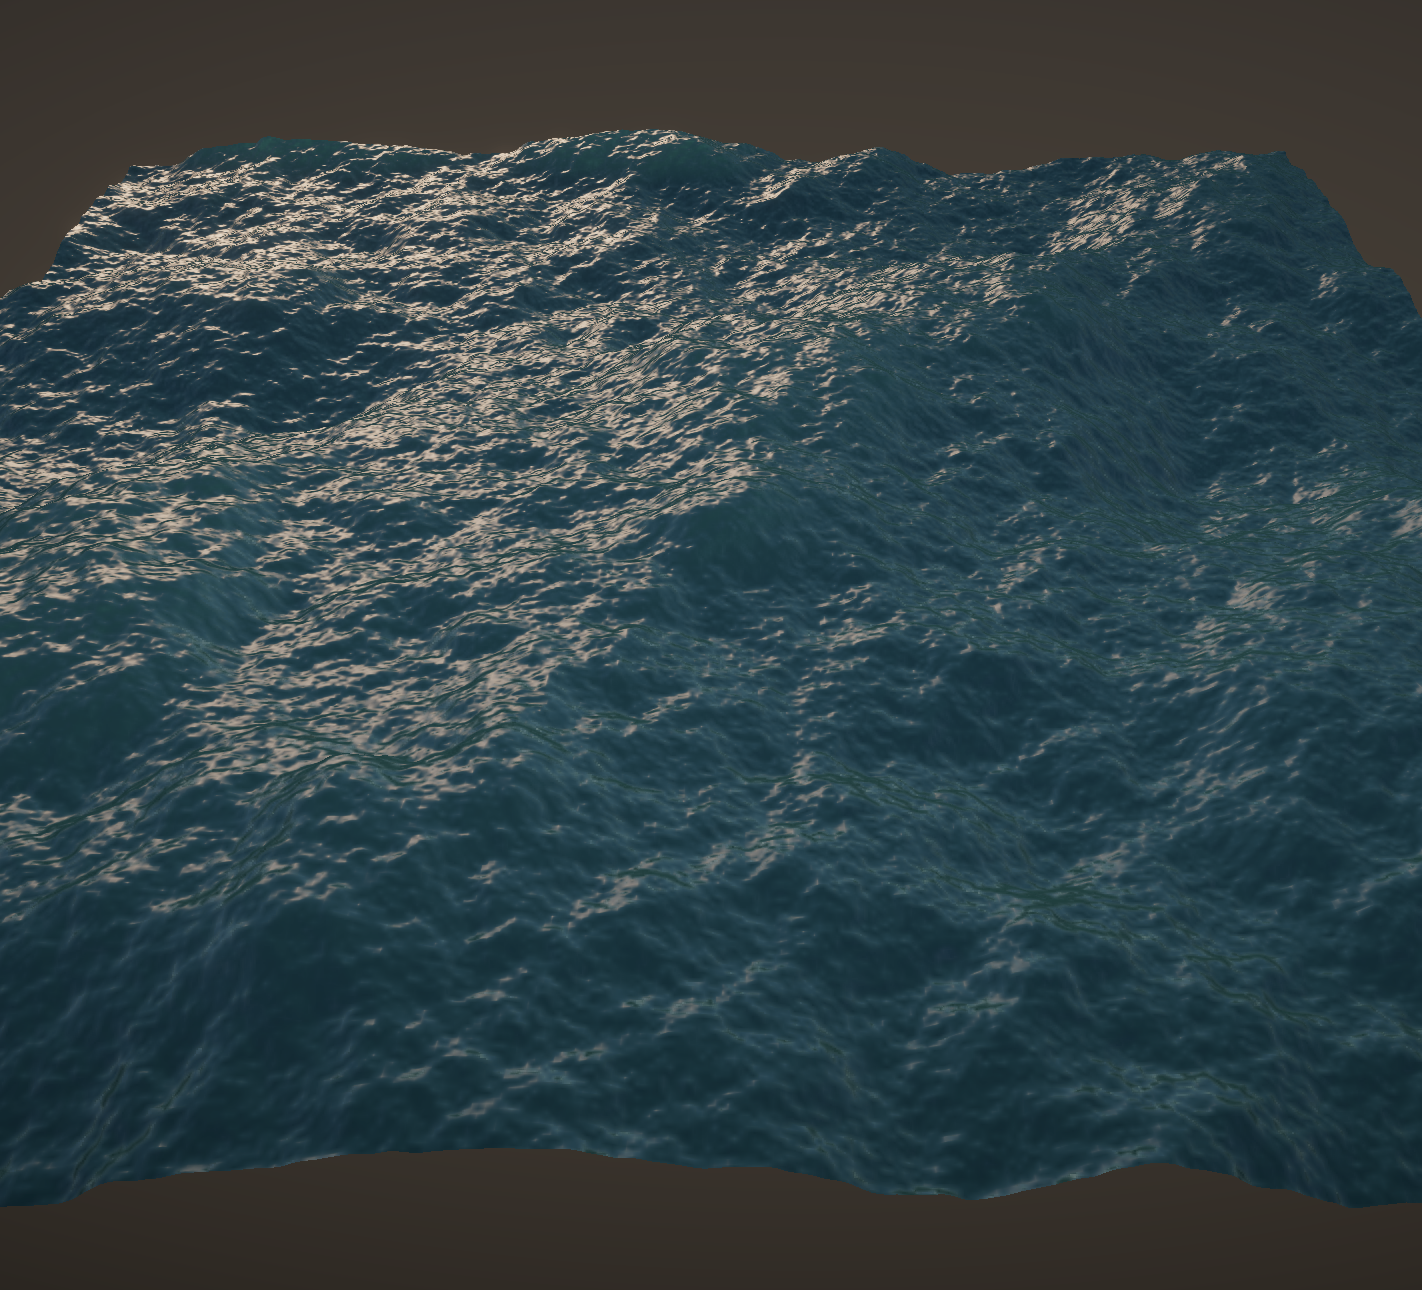
\includegraphics[width=0.8\textwidth]{"images/rendered_height_no_coppy.png"}
    \captionof{figure}{Ocean without Choppy Waves}
    \label{fig:ocean_no_choppy}
\end{minipage}
\begin{minipage}{0.49\textwidth}
    \centering
    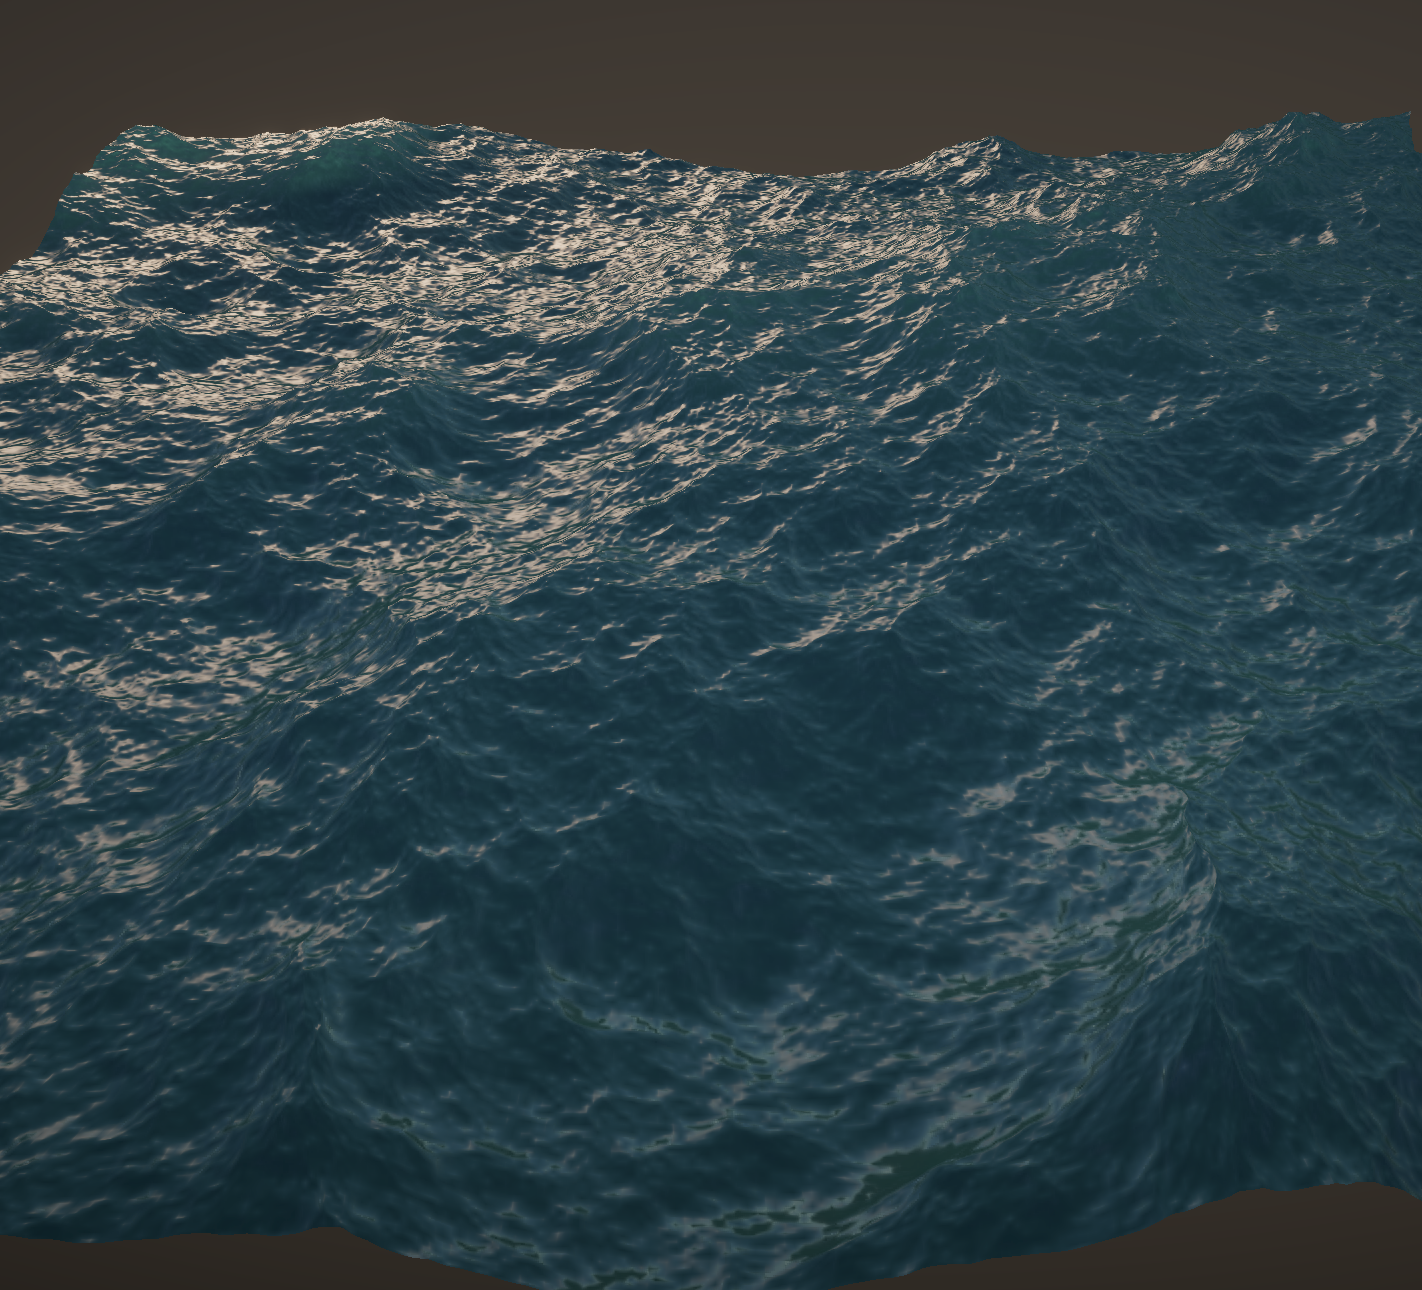
\includegraphics[width=0.8\textwidth]{"images/rendered_height_choppy.png"}
    \captionof{figure}{Ocean with Choppy Waves}
    \label{fig:ocean_choppy}
\end{minipage}
\vspace{0.3cm}

The current rendering of the ocean (Figure \ref{fig:ocean_no_choppy}) appears excessively smooth and lacks the characteristic choppiness of real-world ocean waves. To address this, we introduce horizontal displacement into our model. This not only enhances the choppiness of the waves but also improves the realism of energy transfer between waves (Figure \ref{fig:ocean_choppy}).
The calculation of horizontal displacement follows the formula proposed by Tessendorf (2001) \cite{tessendorf2001}:
\begin{equation}
    \mathbf{D}_{\text{hori}}(\textbf{x}, t) = -i\frac{\mathbf{k}}{k}\tilde{h(\mathbf{k}, t)}
\end{equation}
Utilizing this horizontal displacement, we can adjust the position of our vertices as follows:
\begin{equation}
    \mathbf{x} + \lambda \mathbf{D}_{\text{hori}}(\textbf{x}, t)
\end{equation}
, where $\lambda$ is "choppy factor".
Once again we need to perform IFFT \ref{fig:ifft_algorithm} to get horizontal displacement in the time domain.

\section{Ocean Shading}

\begin{table}[H]
    \centering
    \begin{tabular}{cl|cl}
        \toprule
        \textbf{Symbol} & \textbf{Parameter} & \textbf{Symbol} & \textbf{Parameter} \\
        \midrule
        $L_a$ & Ambient Light & $C_{s}$ & Specular Color \\
        $L_{ss}$ & Subsurface Scatter Light & $C_{ws}$ & Water Scattering Color \\
        $L_s$ & Specular Light & $C_{\text{sky}}$ & Sky Color \\
        $L_r$ & Enviroment Reflection & $H$ & Ocean Height \\
        $N$ & Normal & $F$ & Fresnel Effect \\
        $D_s$ & Sun Direction & $\rho_a$ & Air Bubble Density \\
        $D_v$ & View Direction & $k_a$ & Ambient Light Intensity \\
        $D_i$ & Camera To Fragment Direction & $k_{ss_1}$ & Subsurface Scattering Intensity \\
        $C_a$ & Ambient Light Color & $k_{ss_2}$ & Subsurface Scattering Intensity \\
        $C_l$ & Light Color & $k_{r}$ & Reflection Intensity \\
        $C_b$ & Air Bubble Color & & \\
        \bottomrule
    \end{tabular}
    \caption{Lighting Parameters}
    \label{table:lighting_parameters}
\end{table}

\subsection{Lighting Model}

\subsubsection{Output}

The lighting model employed in our simulation, as shown in Equation \ref{eq:light_model}, is a combination of four fundamental components: ambient light, subsurface scattering, specular light, and environmental reflection. This model is the outcome of integrating the Phong model with concepts derived from the Game Developers Conference “Wakes, Explosions and Lighting: Interactive Water Simulation in Atlas” by Mark Mihelich and Tim Tcheblokov (2021) \cite{mark2021}. The resultant visual output of this composite lighting model can be observed in Figure \ref{fig:output_light}.
\begin{equation}
    L = L_a + L_{ss} + L_s + L_r
    \label{eq:light_model}
\end{equation}
\begin{minipage}{1\textwidth}
    \centering
    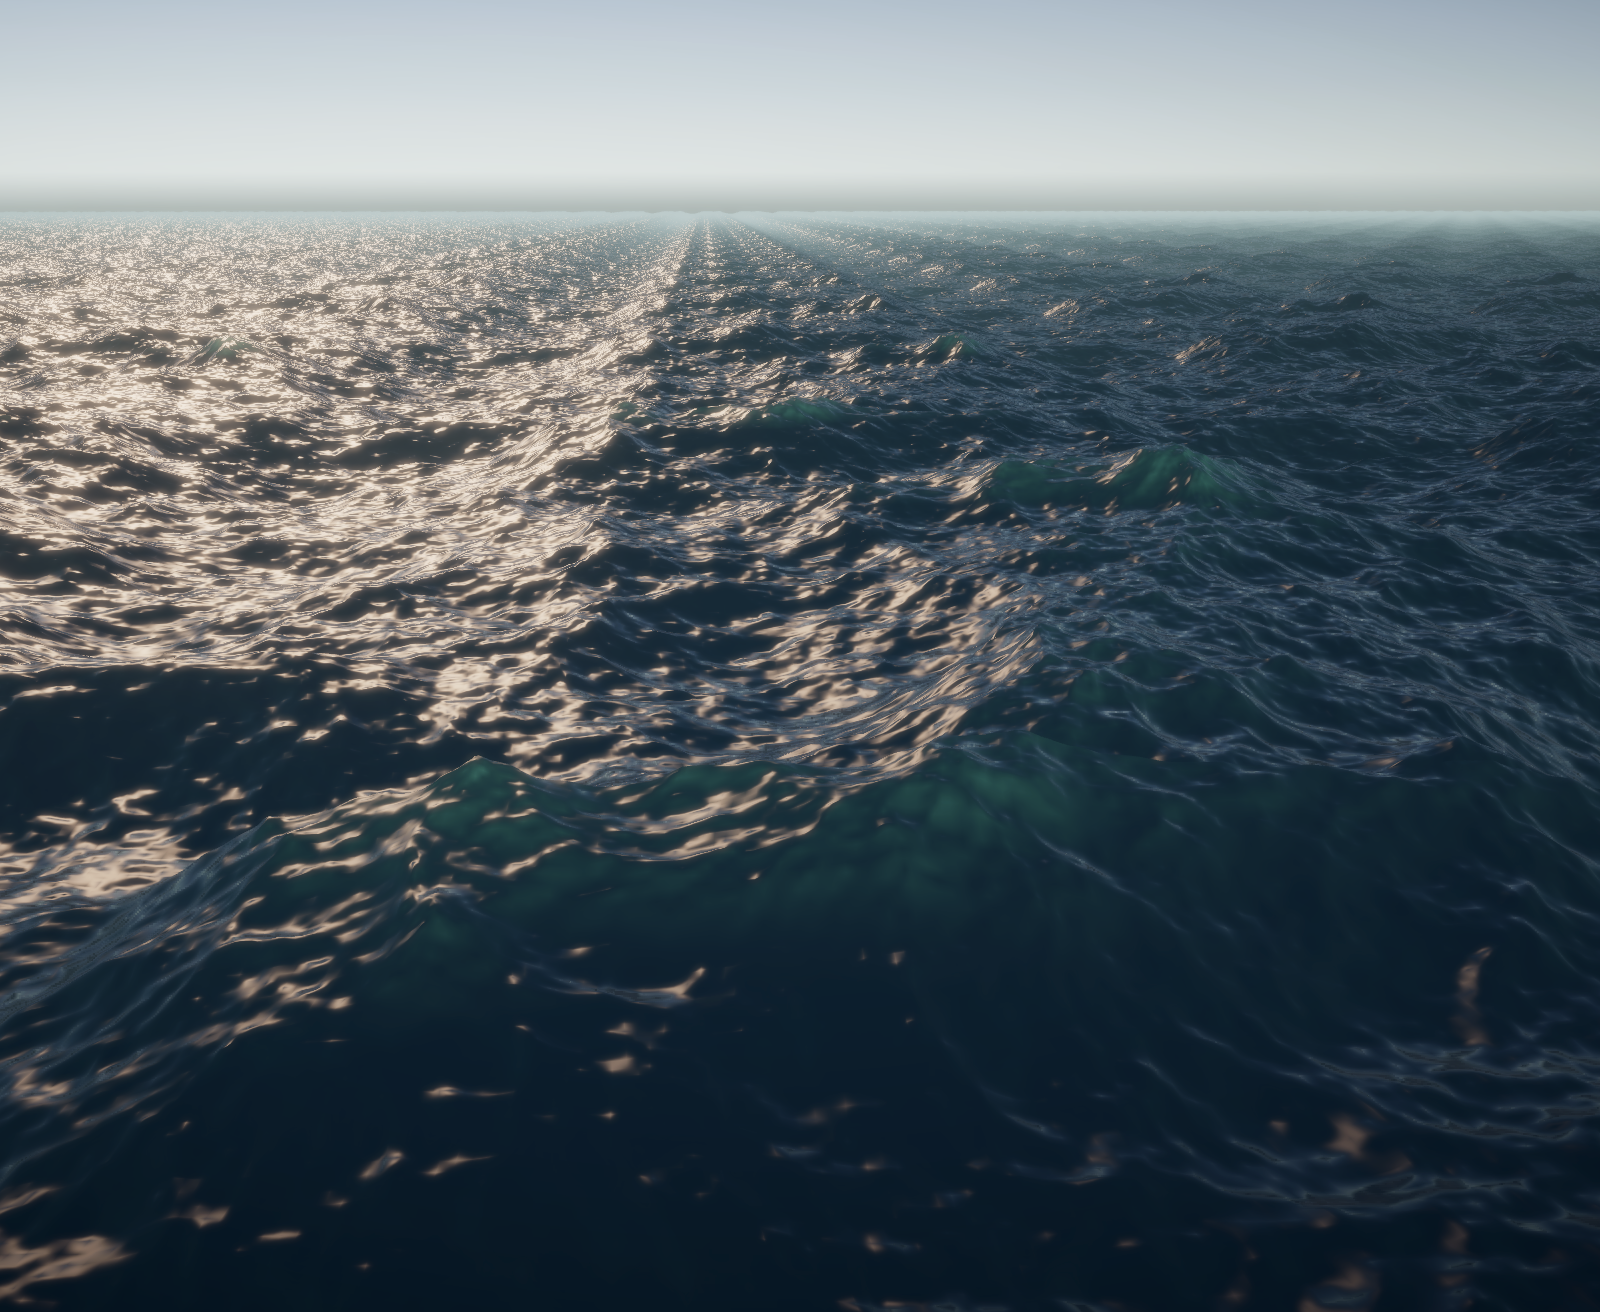
\includegraphics[width=0.50\textwidth]{"images/output_light.png"}
    \captionof{figure}{Finall Shader Output}
    \label{fig:output_light}
\end{minipage}

\subsubsection{Ambient Light}
Ambient light, a constant illumination that does not depend on the direction of the light source, is the result of light scattering in the environment. For oceanic simulations, we utilize an approximation formula for ambient light derived from the GDC conference by Mark Mihelich and Tim Tcheblokov (2021) \cite{mark2021}: 
\begin{equation}
    L_a = k_a N C_a C_l + \rho_a C_b C_l
\end{equation}
\begin{minipage}{1\textwidth}
    \centering
    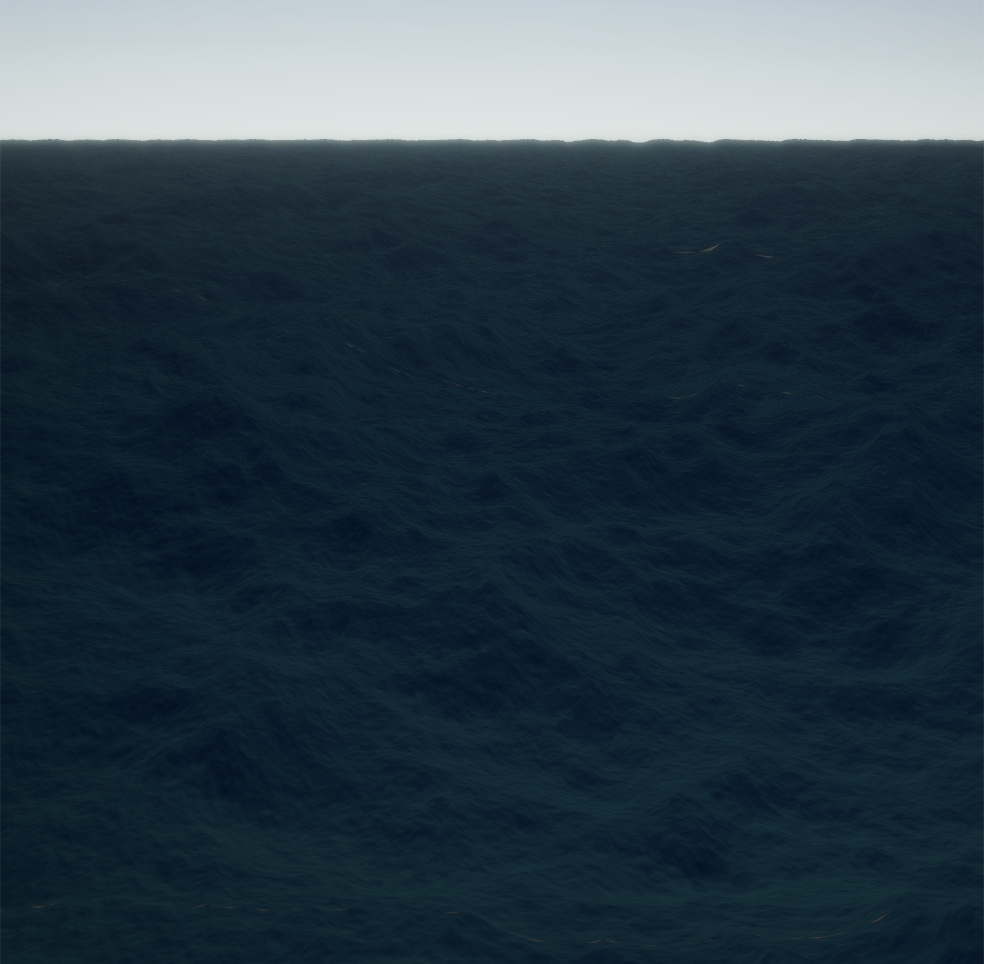
\includegraphics[width=0.40\textwidth]{"images/ambient_light.png"}
    \captionof{figure}{Ambient Light}
    \label{fig:ambient_light}
\end{minipage}

\subsubsection{Fresnel Effect}
The Fresnel effect [TALK ABOUT FRESNEL], a phenomenon where light is more reflective at grazing angles as shown in figure \ref{fig:fresnel_effect}, is crucial for calculations involving specular and reflection:
\begin{equation}
    F = (1 - \max(D_v \cdot N, 0.15))^{5}
\end{equation}
\begin{minipage}{1\textwidth}
    \centering
    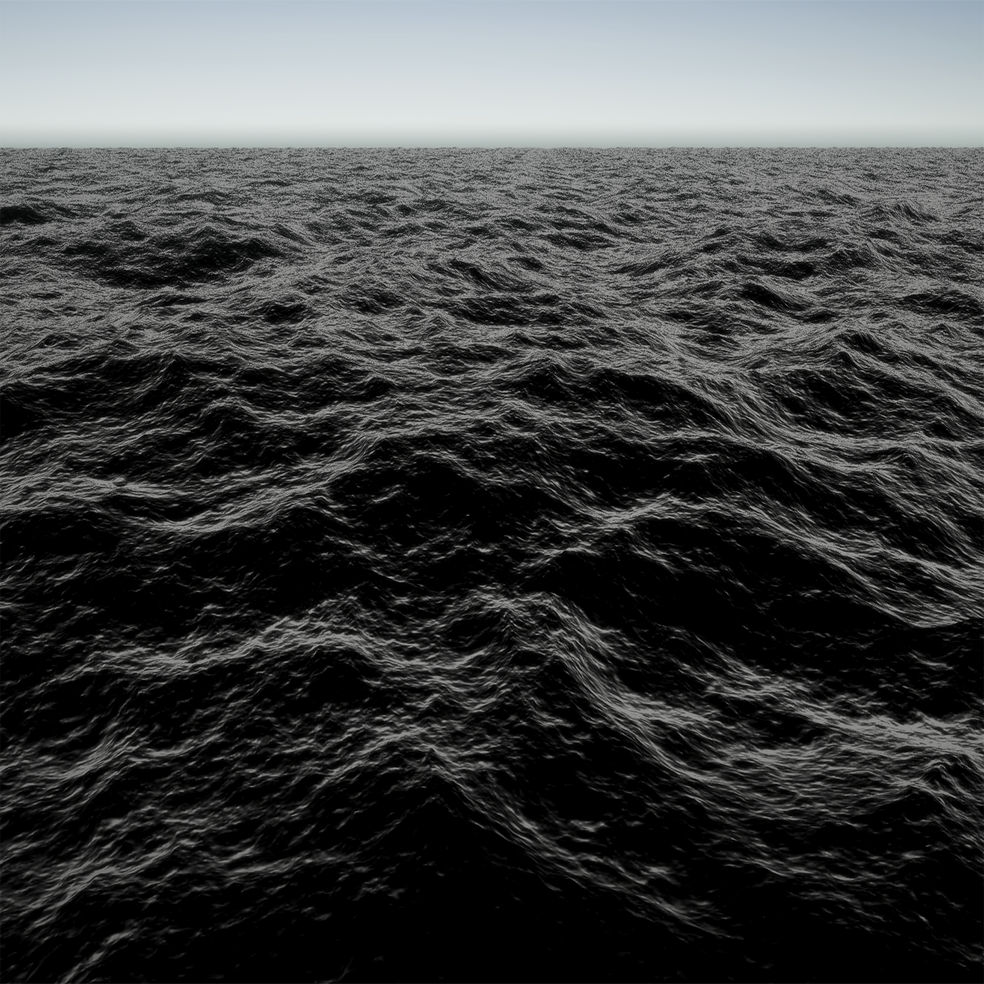
\includegraphics[width=0.40\textwidth]{"images/fresnel.png"}
    \captionof{figure}{Fresnel Effect}
    \label{fig:fresnel_effect}
\end{minipage}

\subsubsection{Subsurface Scattering}

Subsurface scattering describes the interaction of light when it penetrates an object, in this case, water. While ray tracing would typically be required for realistic results, we can use an approximation from the GDC conference [WHAT DO I DO HERE???] \cite{mark2021} due to the majority of our light being trapped in the ocean, with only light at wave peaks able to escape. 
\begin{equation}
    \begin{split}
        L_{ss} &= (1-F) (L_{ss_1} + L_{ss_2}) C_{ws} C_l\\
        L_{ss_1} &= k_{ss_1} \max(0, H) ([D_s, -D_v])^{4}(0.5-0.5(D_s \cdot N))^{3}\\
        L_{ss_2} &= k_{ss_2} ([D_{v}, N])^{2}
    \end{split}
\end{equation}
\begin{minipage}[t]{0.32\textwidth}
    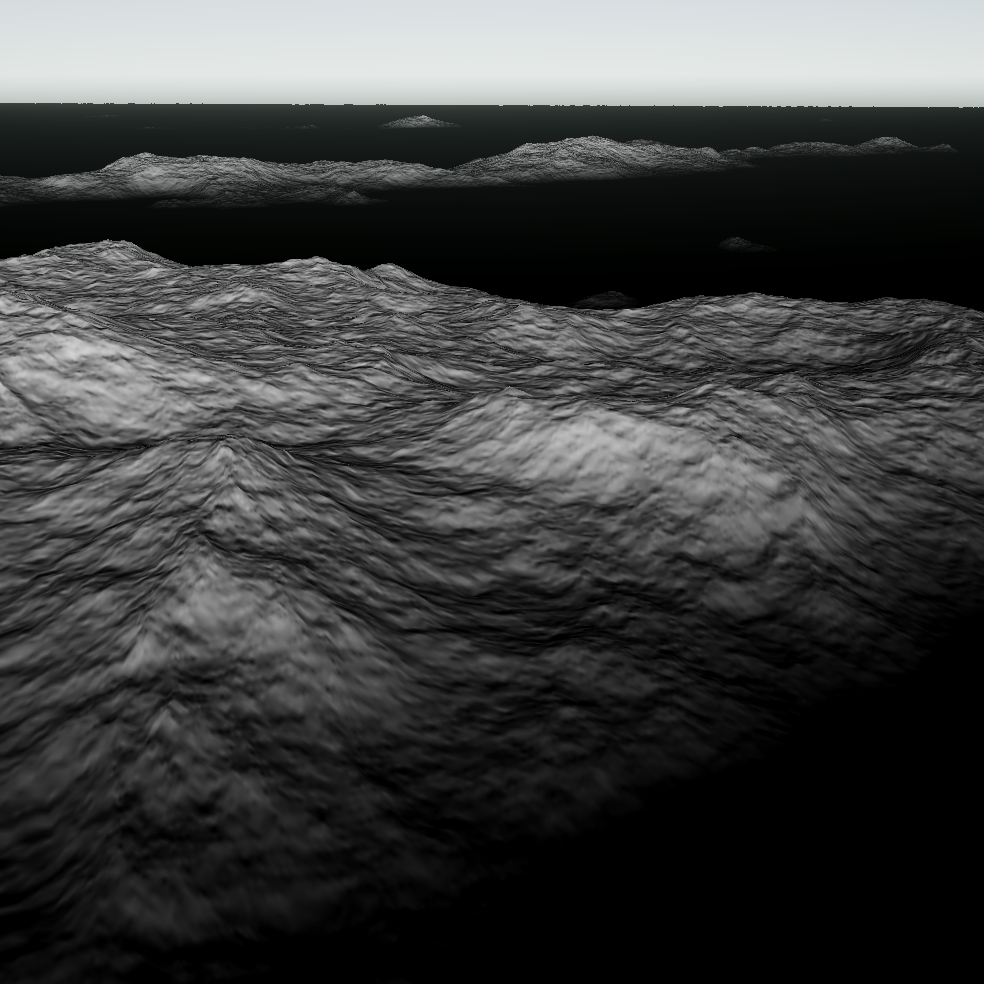
\includegraphics[width=1\textwidth]{"images/ss1_light.png"}
    \captionof{figure}{$L_{ss_1}$}
    \label{fig:lss1_light}
\end{minipage}
\hfill
\begin{minipage}[t]{0.32\textwidth}
    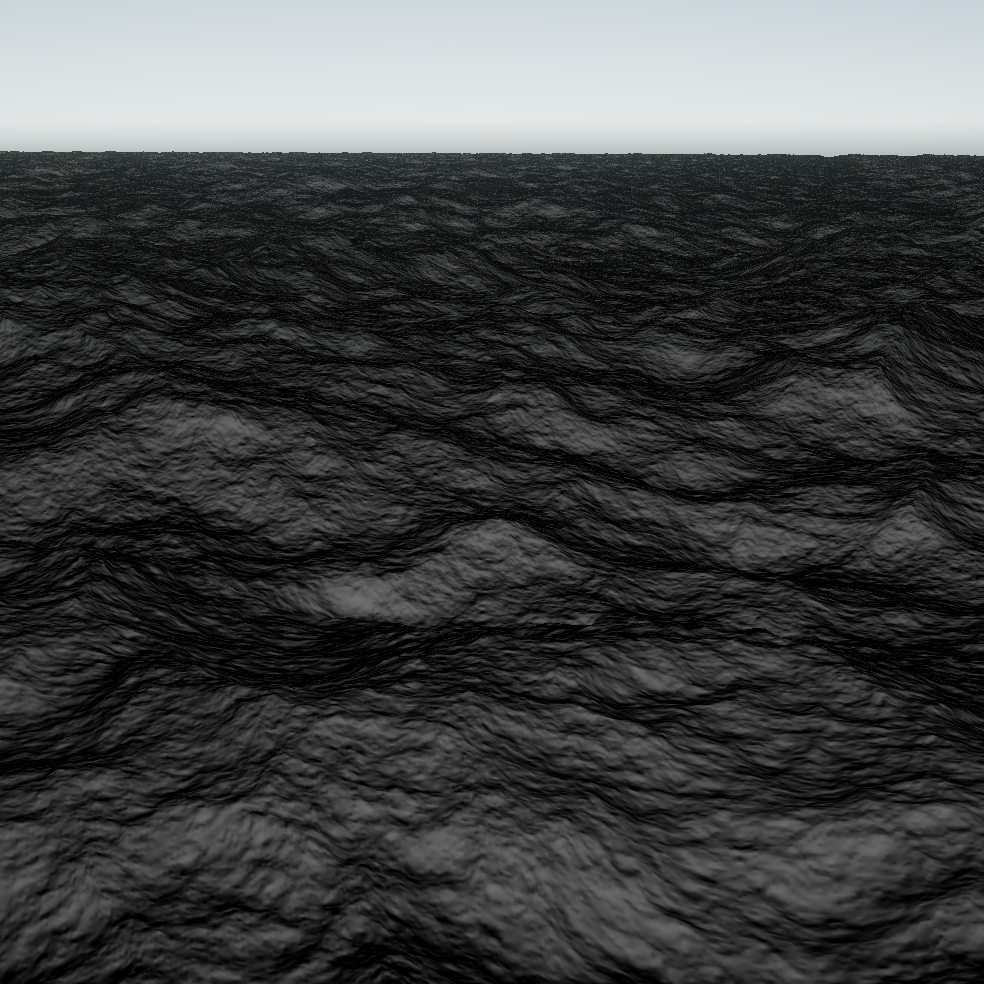
\includegraphics[width=1\textwidth]{"images/ss2_light.png"}
    \captionof{figure}{$L_{ss_2}$}
    \label{fig:lss2_light}
\end{minipage}
\hfill
\begin{minipage}[t]{0.32\textwidth}
    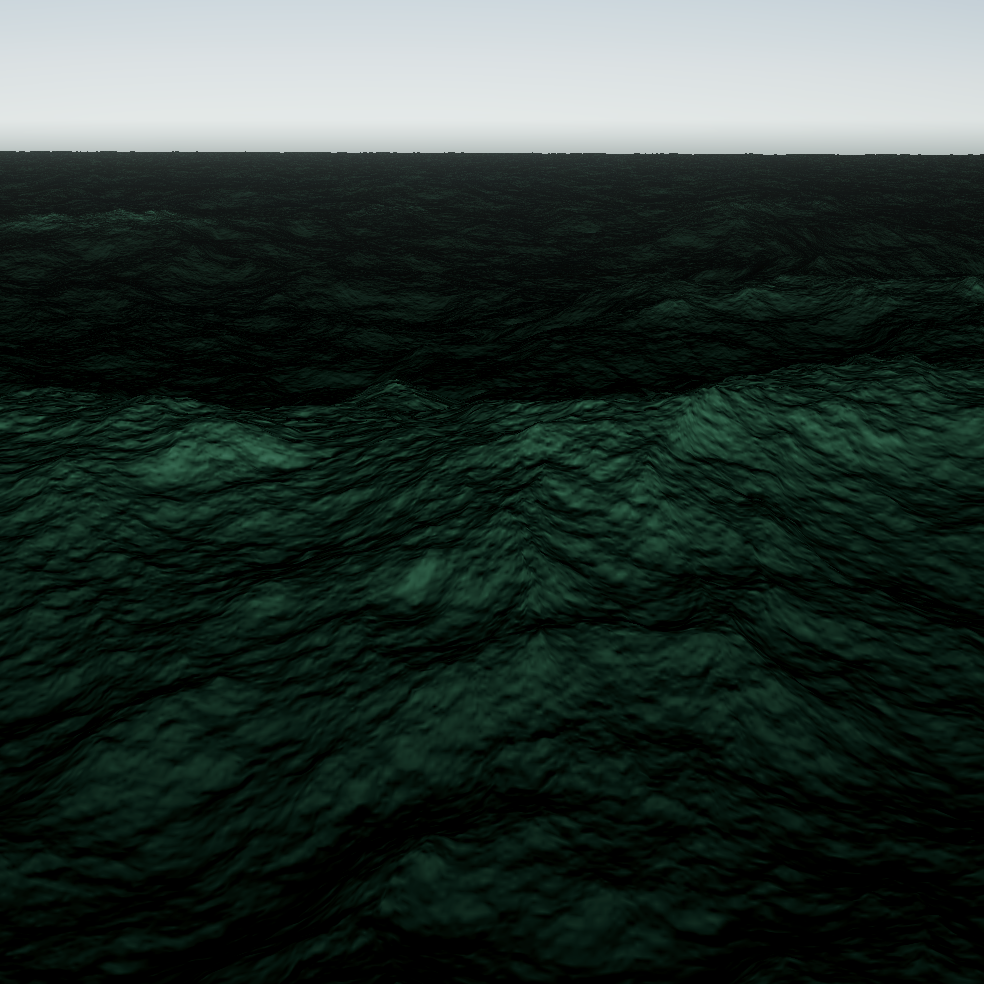
\includegraphics[width=1\textwidth]{"images/ss_light.png"}
    \captionof{figure}{Subsurface Scattering}
    \label{fig:lss_light}
\end{minipage}

\subsubsection{Specular Reflection}
Specular reflection is like the shiny reflection we see on smooth surfaces. It's what makes things like metals, plastics, and in our case water look glossy. In our simulation, we utilize the Phong specular reflection model (Equation \ref{eq:phong_specular}) and incorporate the Fresnel effect, denoted by F. The specular reflection can be observed in Figure \ref{fig:specular_light}.

\begin{minipage}{1\textwidth}
    \centering
    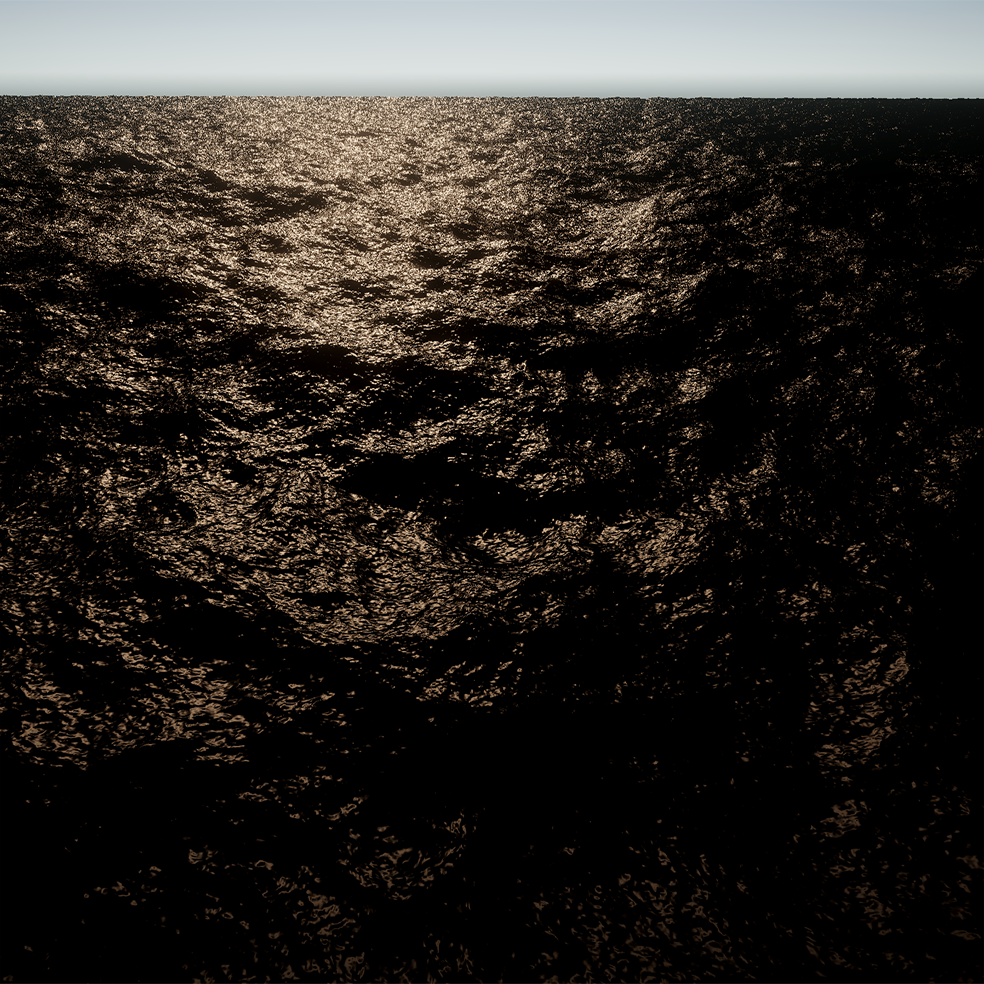
\includegraphics[width=0.45\textwidth]{"images/specular_light.png"}
    \captionof{figure}{Specular Reflection}
    \label{fig:specular_light}
\end{minipage}

\subsubsection{Enviroment Reflection}
In our project, we only consider the reflection of the skybox on the water surface. As per Figure \ref{fig:relfection_light}, we illustrate how skybox reflection operates on a calm ocean surface to better visualize environmental reflection.
\begin{equation}
    \begin{split}
        L_r &= F k_r C_{\text{sky}}\\
        C_{\text{sky}} &= \text{Sky}[\text{reflect}({D_i, N})]
    \end{split}
\end{equation}
\begin{minipage}{1\textwidth}
    \centering
    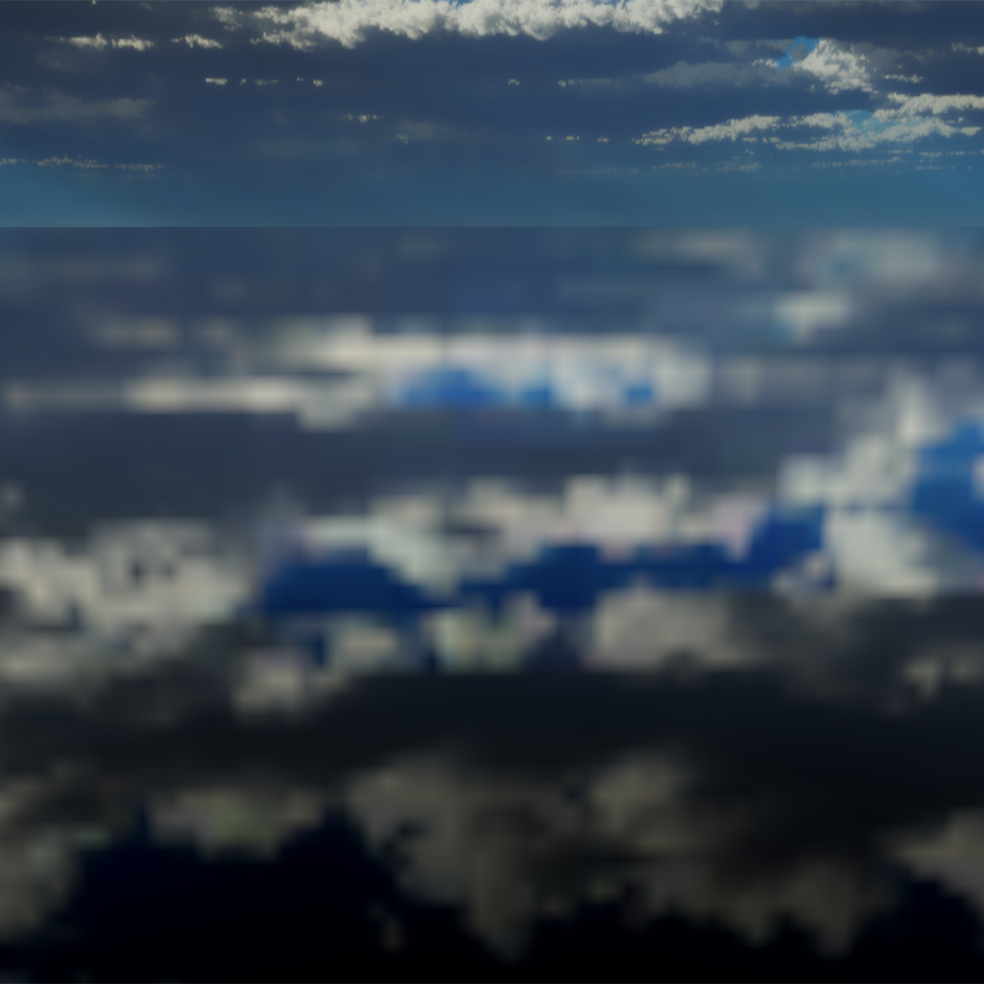
\includegraphics[width=0.45\textwidth]{"images/reflection_light.png"}
    \captionof{figure}{Skybox reflection on calm ocean}
    \label{fig:relfection_light}
\end{minipage}

\subsection{Foam}
\subsubsection{Foam Generation}
\begin{minipage}{1\textwidth}
    \centering
    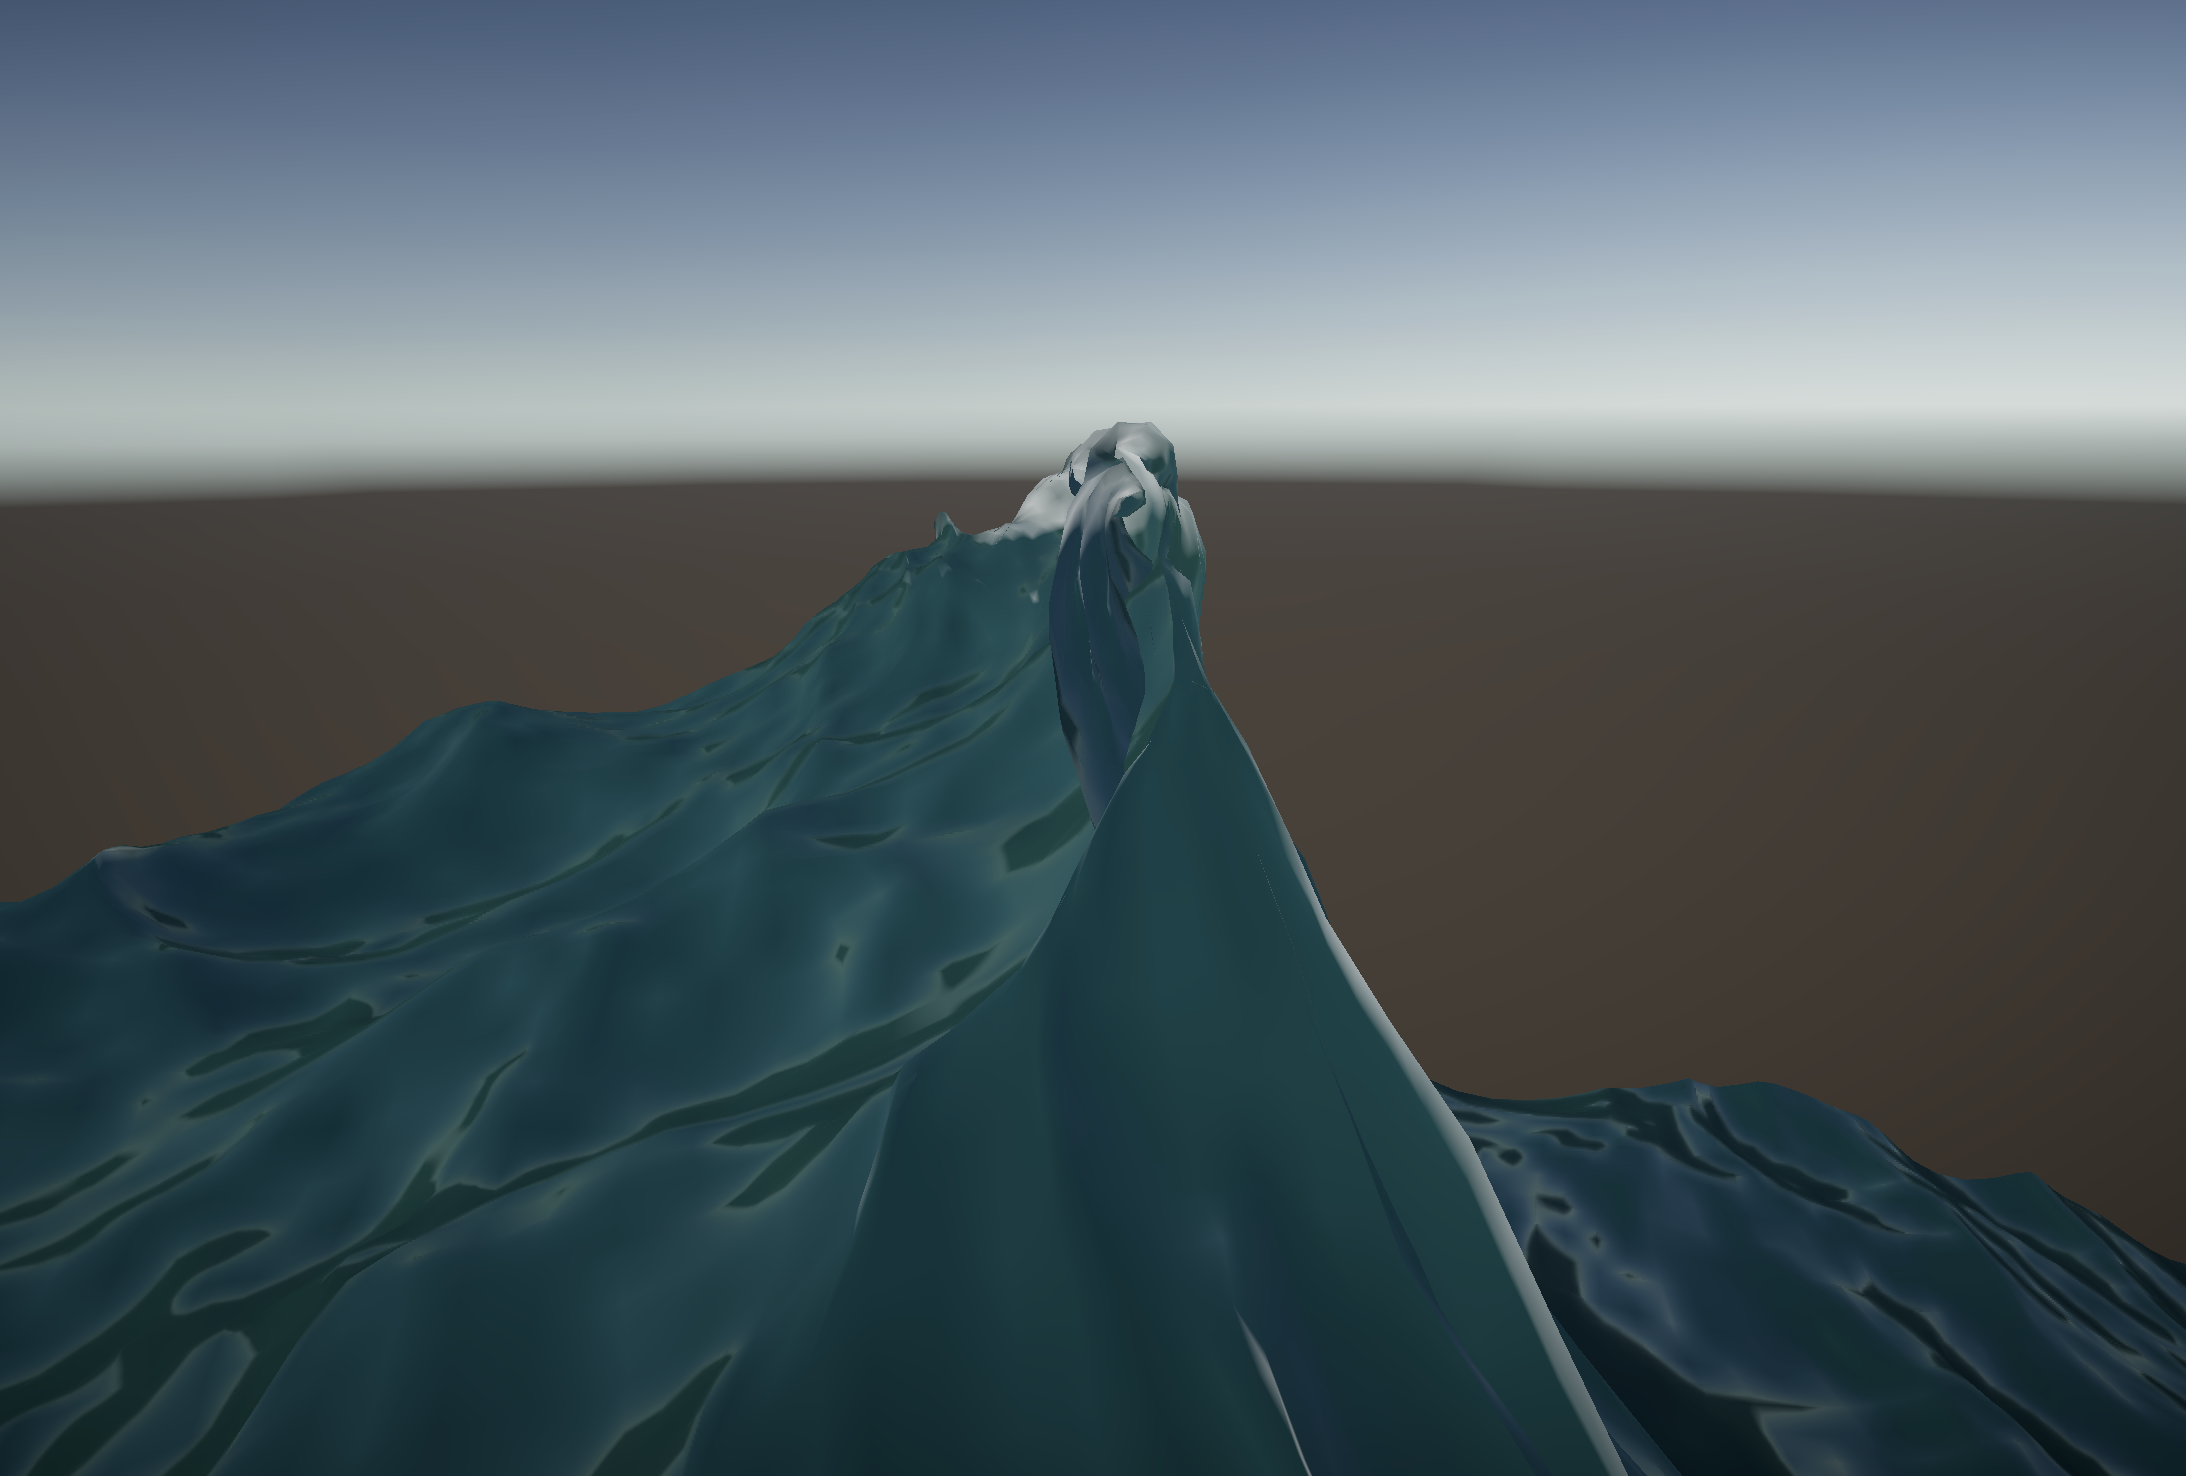
\includegraphics[width=0.50\textwidth]{"images/wave_curl.png"}
    \captionof{figure}{Wave Curl At Wave Peek}
    \label{fig:wave_curl}
\end{minipage}

Ocean foam is a salient and realistic feature of the ocean, contributing to its distinct and authentic appearance. The primary occurrence of foam is observed during wave crashes, a phenomenon facilitated by horizontal displacement. This can be visually discerned at the peaks of waves where the water curls up, as illustrated in Figure \ref{fig:wave_curl}. In essence, our horizontal transformation undergoes an inversion.

As proposed by Tessendorf (2001) \cite{tessendorf2001}, the rendering of foam can be achieved by calculating the determinant of the Jacobian matrix for horizontal displacement, which helps identify these inversions. In our ocean simulation, the Jacobian matrix provides insights into the changes over the x and z axes. When determinant of the Jacobian matrix is bellow zero the "wave crash" happens:

\begin{equation}
    \text{Det}(\mathbf{x}) = J_{xx} + J_{yy} - J_{xy} J_{yx}
\end{equation}
where,
\begin{equation}
    J(\mathbf{x}) = 
    \begin{bmatrix} 
        1 + \lambda\frac{\partial D_x(\mathbf{x})}{\partial x} & 1 + \lambda\frac{\partial D_x(\mathbf{x})}{\partial y} \\
        1 + \lambda\frac{\partial D_y(\mathbf{x})}{\partial x} & 1 + \lambda\frac{\partial D_y(\mathbf{x})}{\partial y} 
    \end{bmatrix} 
\end{equation}
in this case $J_{xy} = J_{yx}$. After appling IFFT, the results can be observed in figure \ref{fig:foam_texture}.

\begin{minipage}{1\textwidth}
    \centering
    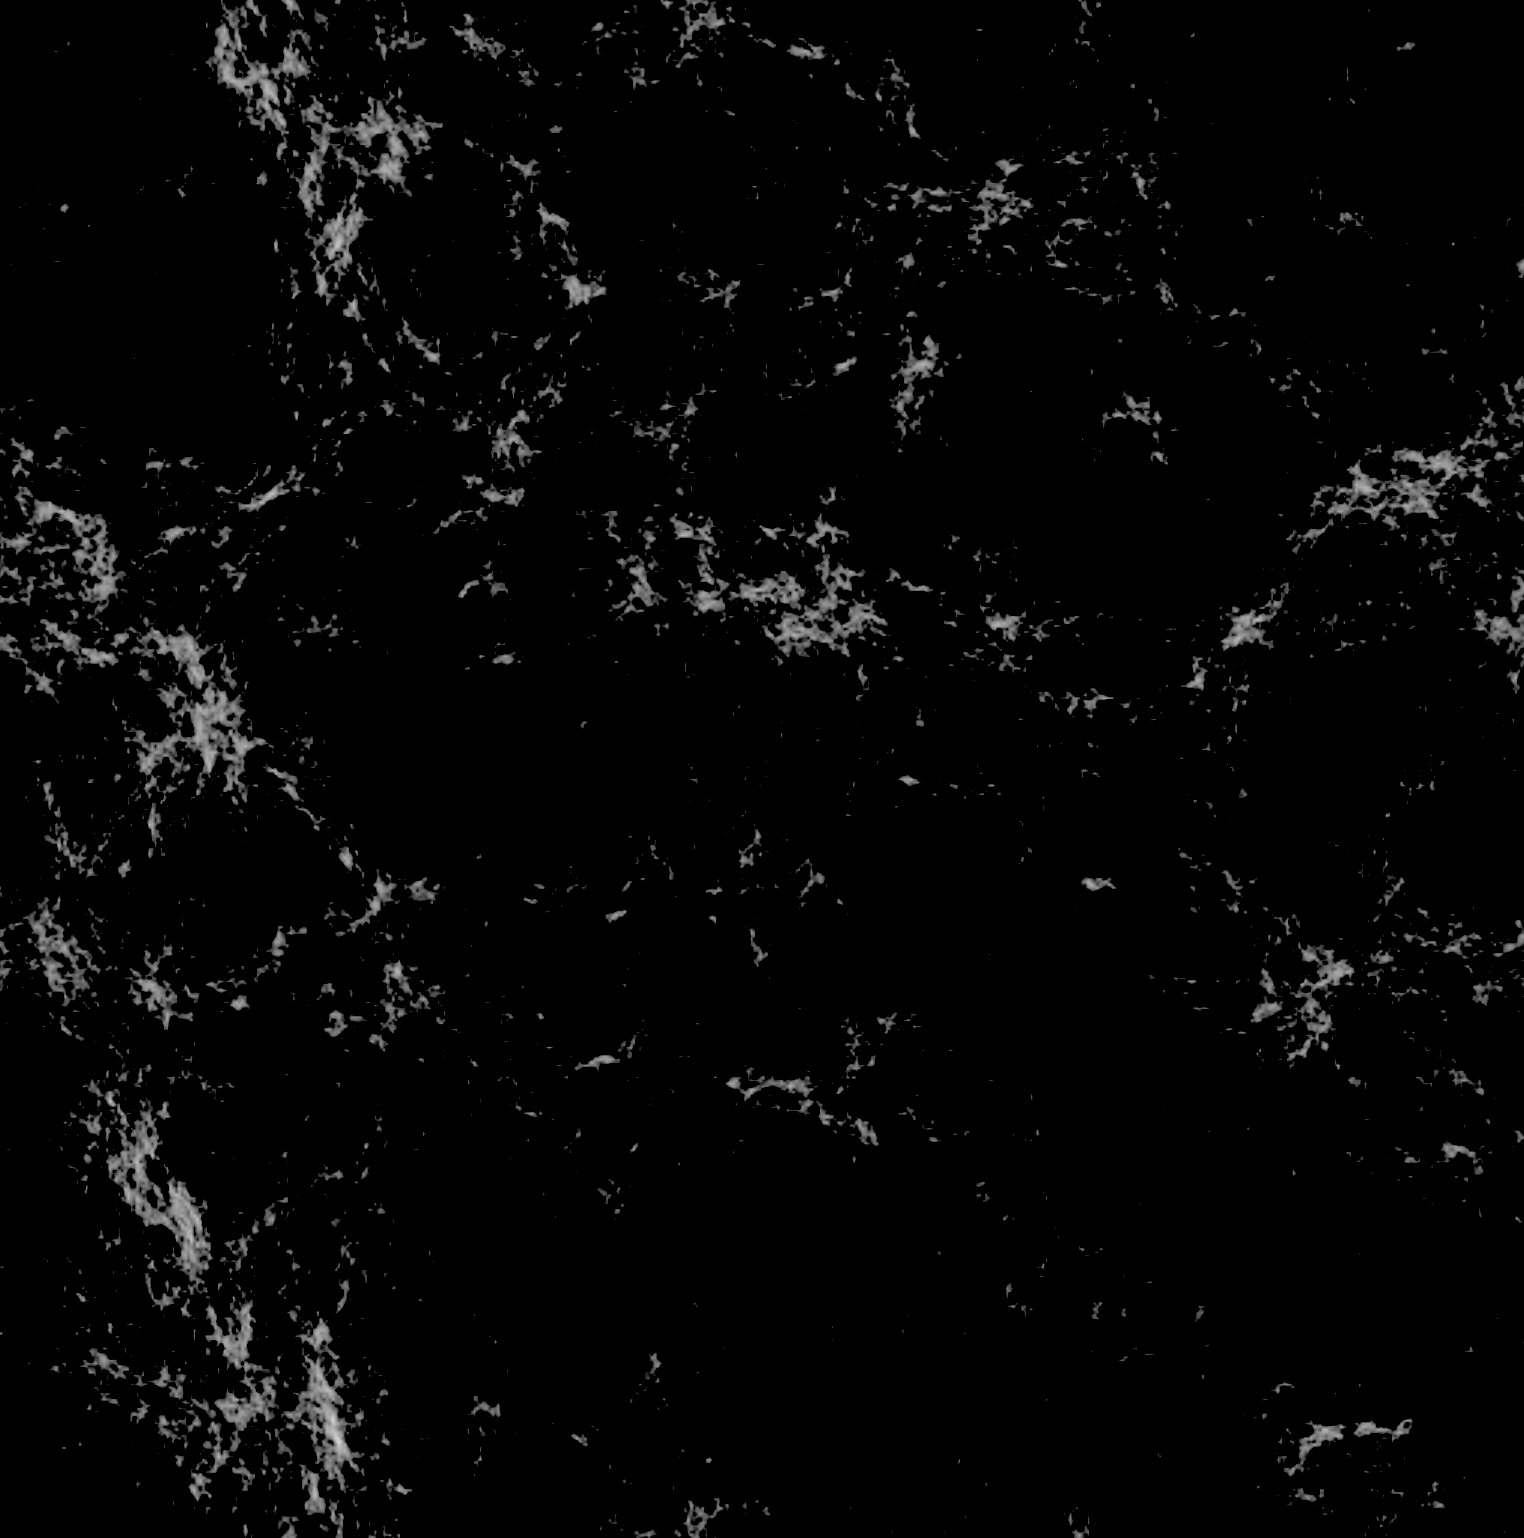
\includegraphics[width=0.40\textwidth]{"images/foam_texture.png"}
    \captionof{figure}{Foam Texture}
    \label{fig:foam_texture}
\end{minipage}

\subsubsection{Foam Accumilation}
Curretlly the foam apears and diasapears quicly, however in real life the foam accumilates and disapears over time.
We can introduce foam accumilation by compering previous and current foam values:
\begin{lstlisting}[caption={Foam Accumilation}, frame=single, numberstyle=\small\color{gray}, captionpos=b]
    accumulation = 
    LastFoamValue - FoamDecay * DeltaTime / max(currentFoam, 0.5);
    foam = max(accumulation, currentFoam);
\end{lstlisting}
This results in pleasing foam accumilation (Figure \ref{fig:ocean_with_foam}):

\begin{minipage}{1\textwidth}
    \centering
    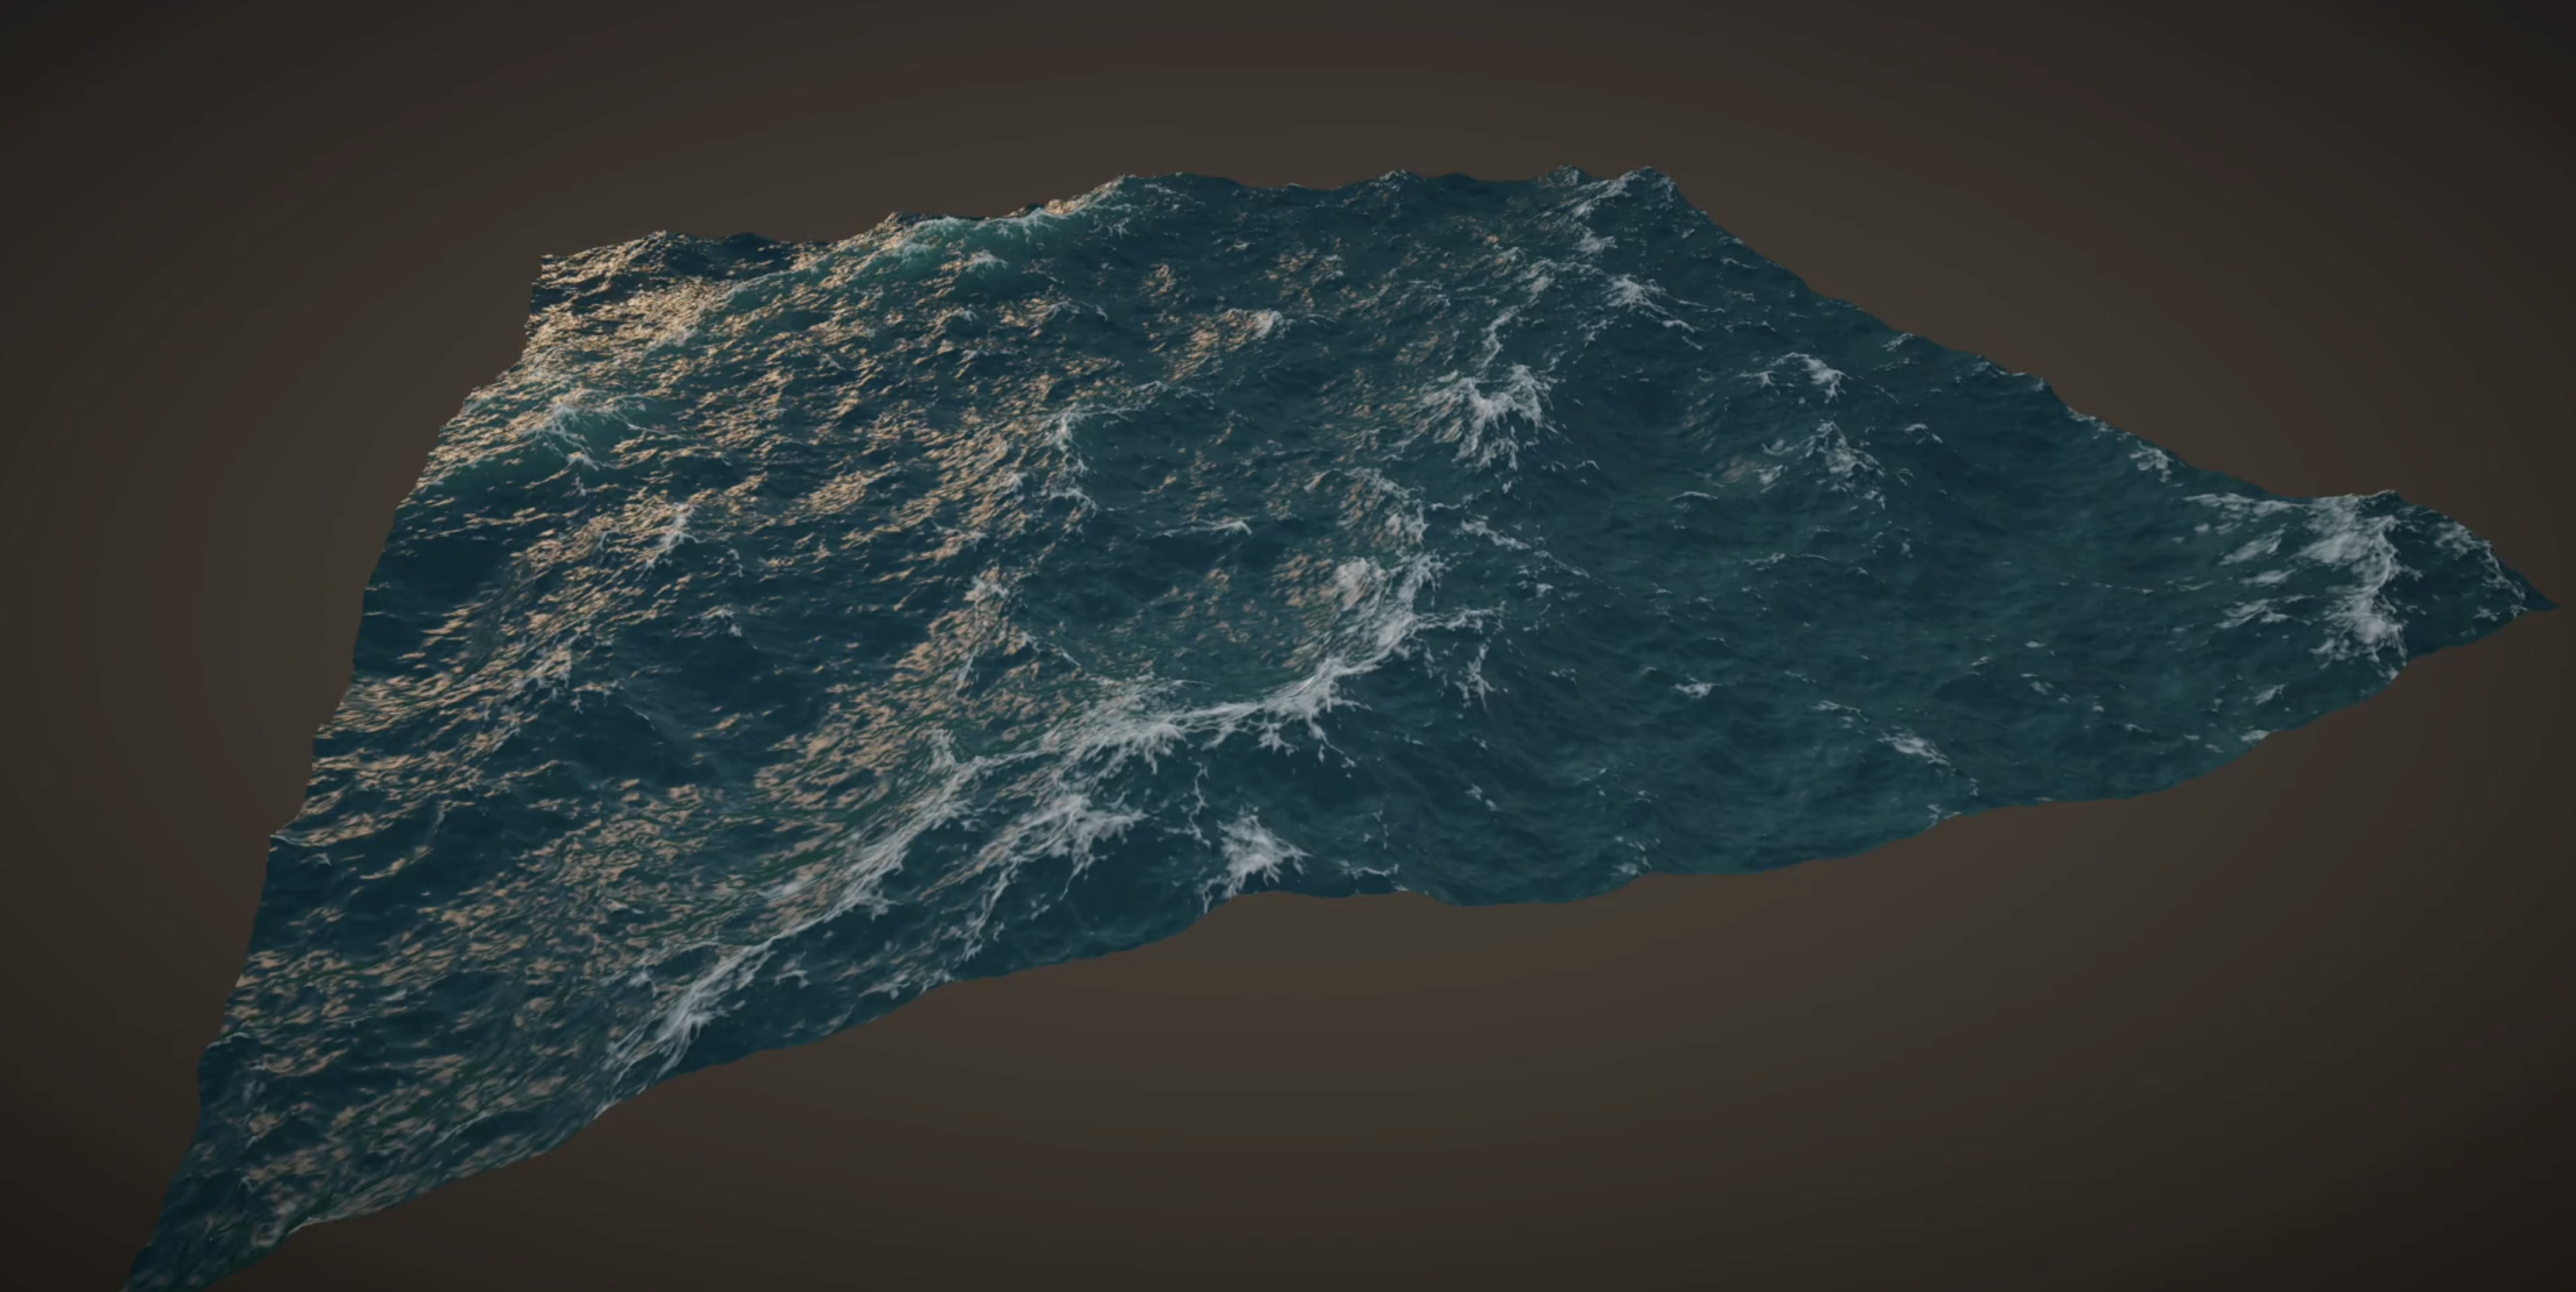
\includegraphics[width=0.8\textwidth]{"images/ocean_with_foam.png"}
    \captionof{figure}{Ocean With Foam}
    \label{fig:ocean_with_foam}
\end{minipage}

\section{Multiple Cascades}
At this stage our ocean with texture 512x512 simulates 262,144 distinc waves however the tilling is still noticible \ref{fig:ocean_with_tilling}.

\begin{minipage}{1\textwidth}
    \centering
    \includegraphics[width=0.8\textwidth]{"images/tilling_ocean.png"}
    \captionof{figure}{Ocean with Tilling, using 512x512 texture}
    \label{fig:ocean_with_tilling}
\end{minipage}

To counter this we could increase our simulation texture however even FFT becomes expensive really fast.
Another approuch is to simulate multiple cascades for diffrent wave lengths $k$ \ref{fig:cascades} and diffrent $l$ length scales. We can split our simulation into 3 parts, big waves, medium waves and small waves.

\begin{minipage}{1\textwidth}
    \centering
    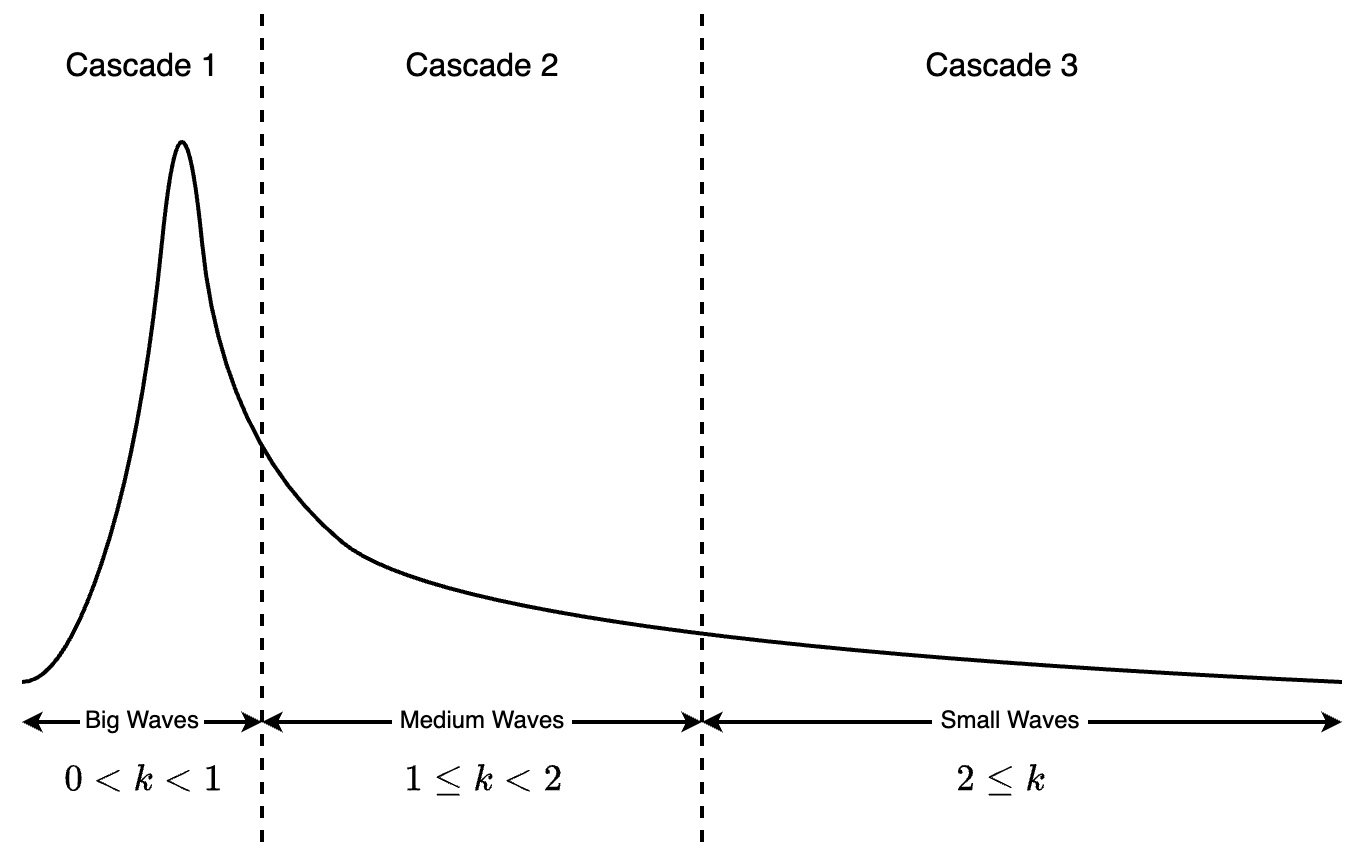
\includegraphics[width=0.8\textwidth]{"images/cascades.png"}
    \captionof{figure}{Cascades [EXPLAIN MORE???]}
    \label{fig:cascades}
\end{minipage}

When it comes to chosing $l$ we need to follow these steps:
\begin{enumerate}
    \item We chose bigger $l$ for bigger waves as we are more likly to notice tilling with big waves
    \item We chose smaller $l$ for smaller waves as we are less likly to notice tilling with small waves
\end{enumerate}
This results ocean that has less tilling and more detail \ref{fig:ocean_with_cascades}.

\begin{minipage}{1\textwidth}
    \centering
    \includegraphics[width=0.8\textwidth]{"images/ocean_with_cascades.png"}
    \captionof{figure}{Ocean with Cascades, using 3x(512x512) textures}
    \label{fig:ocean_with_cascades}
\end{minipage}

One of the main pros of having multiple cascades is reduction in performance cost, as we can have similar results of 512x512 with 3x(256x256) textures as shown in figure \ref{fig:ocean_with_cascades_256}.

\begin{minipage}{1\textwidth}
    \centering
    \includegraphics[width=0.8\textwidth]{"images/ocean_cascades_256.png"}
    \captionof{figure}{Ocean with Cascades, using 3x(256x256) textures}
    \label{fig:ocean_with_cascades_256}
\end{minipage}

\section{Library Choice}

In the context of our ocean generation project, we evaluated six potential technologies, which can be categorized into three groups: older APIs, modern APIs, and game engines.

The older APIs category includes OpenGL, an ideal API for learning and cross-platform use. It’s relatively easy to use, but it’s becoming outdated.

The second category, modern APIs, includes Metal, Vulkan, and DirectX. These APIs are more complex to use, but they provide more control over the GPU and lower CPU usage. However, Metal and DirectX are limited to Apple and Microsoft platforms, respectively. In the case of Vulkan, it requires significantly more code to accomplish the same task.

The final category is game engines, specifically Unity and Unreal. These engines are excellent for computer graphics as they offer a wealth of functionality, most importantly, useful UI tools that make development easier. However, they are massive tools with many custom needs, and you need experience to use them correctly.

All these options are viable as they all have the capability to fulfill our project requirements. However, after careful consideration, we chose Unity. his choice was primarily driven by our greater familiarity with Unity compared to other tools. Furthermore, Unity offers a comprehensive suite of tools, encompassing UI design, GPU programming, and an integrated build system. These features significantly streamline the development process, rendering Unity as the optimal choice for our project's needs.

\section{Utilization of Unity Tools}
In our project, we strategically employed Unity’s toolset. We used C\# for startup computations, setting the initial conditions and parameters for our project including communication between CPU and GPU.

For the intensive mathematical computations inside compute shaders and vertex and fragment shaders, we utilized the High-Level Shading Language (HLSL) for GPU programming. This approach allowed us to leverage the computational power of the GPU, enhancing the performance and visual fidelity of our project.

Additionally, Unity’s built-in User Interface (UI) system and build system were used for creating interactive UIs and streamlining the compilation process, respectively. These tools collectively contributed to the effective and efficient development of our project.

\section{Version Controll}
In the development of our project, we adopted GitHub as our version control system. This platform facilitated the systematic management of different versions of our project files. By organizing our project into branches, we were able to work on individual features without affecting the main codebase. This approach not only enhanced the efficiency of our development process but also ensured the integrity and stability of our project.
